\subsection{Nascent IFIT Interaction with RSV Inclusion Bodies} \label{subsec:Nascent IFIT Interaction with RSV Inclusion Bodies}
\subsubsection{Phenotypic Diversity of Nascent IFIT1 Interaction with RSV IBs}
Initial experiment suggested hIFIT1 colocalises with the hRSV IBs in A549 cell line, however assessing all 281 observation we can see that hIFIT1 displays a range of phenotypic divesity with regards to interaction with these structures. As can be seen in Figure \ref{fig:Phenotypic Diversity of hIFIT1 Interactions with hRSV Inclusion Bodies in A549 Cell Line}, panel (a), 30\% of interactions result in either full or partial exclusion from the structure or an even diffusion through the IB and the surroinding cytosol. Next most common phenotype is a inclusion inside the IB structure, occuring in circa 18\% of observation. Following phenotypes, orrucing in the same frequency of 9\%, are a phenotype of colocalisation with the edge of the inclusion body joined with exclusion from the area of the IB; and a edge exclusion phenotype, where IFIT1 was present equaly between the IB and the surrounding cytoplasm with the exeption of of the IB boundry, where its signal is decreased. Representative images of the phenotypes mentioed above can be seen in Figure \ref{fig:Representative Images of Phenotypic Diversity of hIFIT1 Interactions with hRSV Inclusion Bodies in A549 Cell Line}. We have also observed IFIT1 to dysplay edge exclusion with obvoius spots within the IB structure (Edge exclusion + IBAG) and also a colocalisation with phenotype but neither had a sufficiently high frequency of occurance where we can be certain that these are indeed relevant during infection and not just imaging artefacts. In Figure \ref{fig:Phenotypic Diversity of hIFIT1 Interactions with hRSV Inclusion Bodies in A549 Cell Line} panel (b), we can observe the measured areas of the IBs associated with phenotypes which had the frequency of accurance higher than 5\%. We can see that the two most common pheotypes, exclusion and diffusion, had median IB area sizes of 5 and 4.4 \(\mu \mbox{m}^2\), values either identical or very similar to the aggregated median IB area of all the observations in A549 cell line. Both phenotypes also encompass a range of IB sizes, from sub 1 \(\mu \mbox{m}^2\) until supra 20 \(\mu \mbox{m}^2\) IB areas. On the other hand, the other phenotyes observed are more prevalent in larger inclusion bodies. In more detail, inclusion phenotype was more prevalent in supra 3 \(\mu \mbox{m}^2\) inclusion bodies, with the median size of 8; colocalisation accompanied by exclusion phenotype median IB size was 12 \(\mu \mbox{m}^2\), although some IBs with sizes between 0.8 to 5 \(\mu \mbox{m}^2\) showed this phenotype as well; and the edge exlusion phenotype was in IBs with median size of 7 \(\mu \mbox{m}^2\), although these IB were clustered in two clusters with median values of approximately 5 and 10 \(\mu \mbox{m}^2\) respectively. Our data indicates that while in majrity of cases IFIT1 is either excluded or diffused throught the IB structures, regardless ofn the IB size and thus maturity, we can see a potential interaction with more mature IBs of sizes above 5 \(\mu \mbox{m}^2\), which in the literature, coinsides to the IB sizes which have IBAGs present (\cite{Rincheval2017FunctionalVirus}). 

\begin{figure}
    \begin{subfigure}{0.495\textwidth}
        \caption{}
        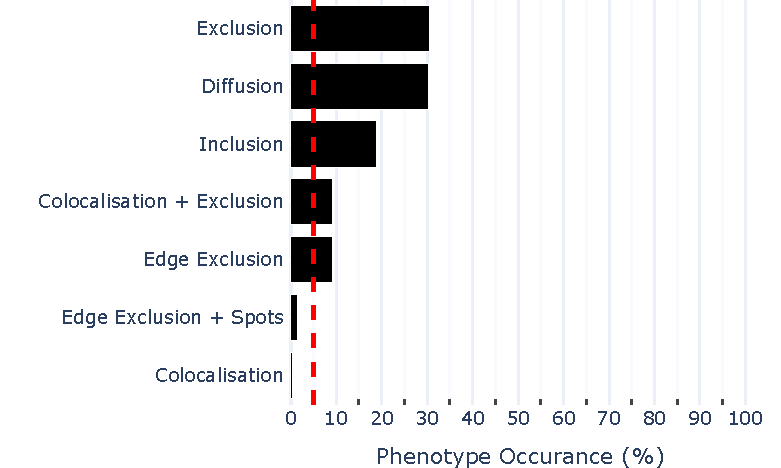
\includegraphics[width=1\linewidth]{08. Chapter 3/Figs/02. Infection/01. IFIT1/01. bar_i1_a549.pdf} 
    \end{subfigure}
    \begin{subfigure}{0.495\textwidth}
        \caption{}
        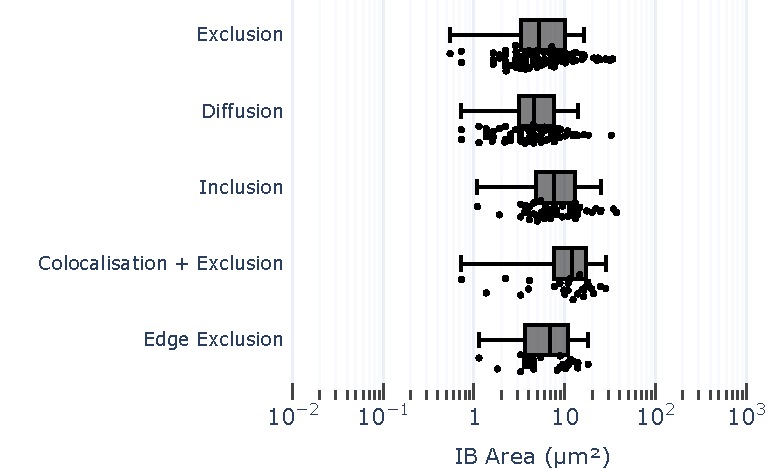
\includegraphics[width=1\linewidth]{08. Chapter 3/Figs/02. Infection/01. IFIT1/02. box_i1_a549.pdf}
    \end{subfigure}
    \caption[Phenotypic Diversity of hIFIT1 Interactions with hRSV Inclusion Bodies in A549 Cell Line.]{\textbf{Phenotypic Diversity of hIFIT1 Interactions with hRSV Inclusion Bodies in A549 Cell Line.} A549 cells were infected with human RSV at MOI 1 and fixed 24 HPI. Cells were double-labeled with with anti-RSV N and anti-IFIT1 antibodies and imaged on confocal microscope. Panel (a) shows percentual proportions of observed phenotypes between hRSV inclusion bodies and hIFIT1 (281 observations), with the red dotted line denoting the 5\% threshold, marking phenotypes considered relevant above this limit. Panel (b) shows the IB area in \(\mu \mbox{m}^2\) per observed relevant phenotype.}
    \label{fig:Phenotypic Diversity of hIFIT1 Interactions with hRSV Inclusion Bodies in A549 Cell Line}
\end{figure}

\begin{figure}
    \centering
    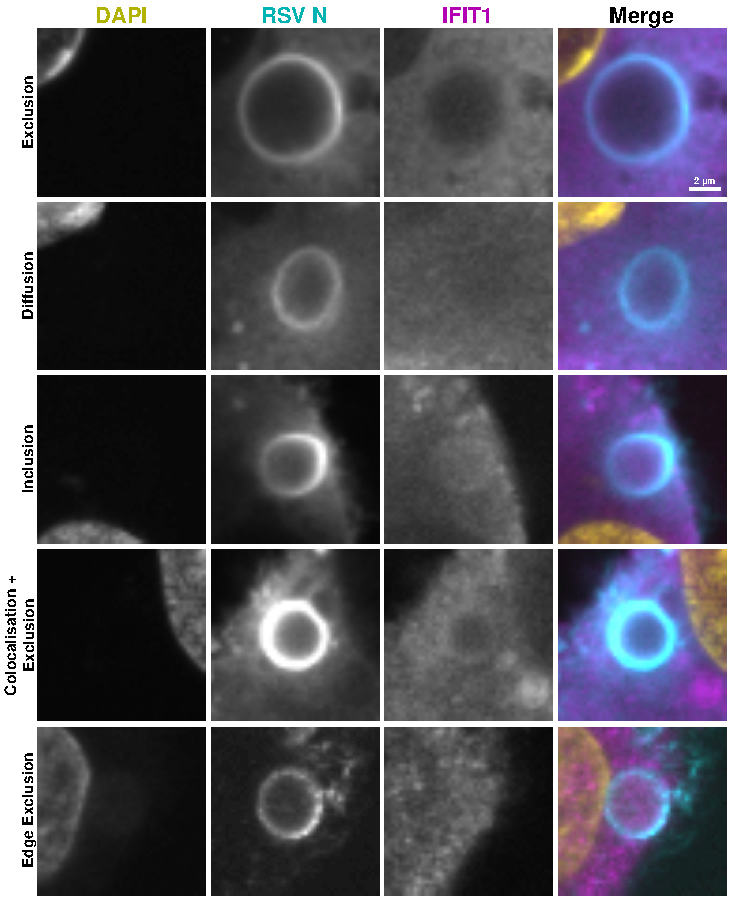
\includegraphics[width=1\linewidth]{08. Chapter 3/Figs/02. Infection/01. IFIT1/03. a549 i1.pdf}
    \caption[Representative Images of Phenotypic Diversity of hIFIT1 Interactions with hRSV Inclusion Bodies in A549 Cell Line.]{\textbf{Representative Images of Phenotypic Diversity of hIFIT1 Interactions with hRSV Inclusion Bodies in A549 Cell Line.} A549 cells were infected with hRSV at MOI 1 and fixed at 24 HPI. Cellular nuclei were stained with DAPI (yellow), and cells were double-labeled with anti-RSV N (cyan) and anti-IFIT1 (magenta) antibodies. This figure showcases representative examples of relevant phenotypes in the interaction between hIFIT1 and hRSV inclusion bodies. These phenotypes are presented in descending order based on their percentage proportions. The scale bar indicates 2 \(\mu \mbox{m}\).}
    \label{fig:Representative Images of Phenotypic Diversity of hIFIT1 Interactions with hRSV Inclusion Bodies in A549 Cell Line}
\end{figure}

We set to validate the previous data in the BEAS2B cell line. Figure \ref{fig:Phenotypic Diversity of hIFIT1 Interactions with hRSV Inclusion Bodies in BEAS2B Cell Line} shows the 45 observed IFIT1/IB interaction phenotypes, their occurance (panel a) and the underlying IB sizes (panel b), while Figure \ref{fig:Representative Images of Phenotypic Diversity of hIFIT1 Interactions with hRSV Inclusion Bodies in BEAS2B Cell Line} shows the respresentative images of phenotypes with the occurance of above 5\%. The majority of observations showed IFIT1 to be either partially or fully excluded from the hRSV inclusion bodies (circa 85\% of observations), while 8\% of phenotypes were diffusion and 4\% displayed colocalisation cojoined with exclusion. The size range of IB from which IFIT1 was exclude mimic the aggregate distribution of all IBs detected within BEAS2B cells, having the equal median size value of 3 \(\mu \mbox{m}^2\) and spread from sub 1 \(\mu \mbox{m}^2\) IBs to supra 10 \(\mu \mbox{m}^2\) ones. The second most common phenotype and the only other that surpassed 5\% of total accurance was diffusion phenitipe, which was observed only in smaller IBs, with the median size of 0.5 \(\mu \mbox{m}^2\).

\begin{figure}
    \begin{subfigure}{0.495\textwidth}
        \caption{}
        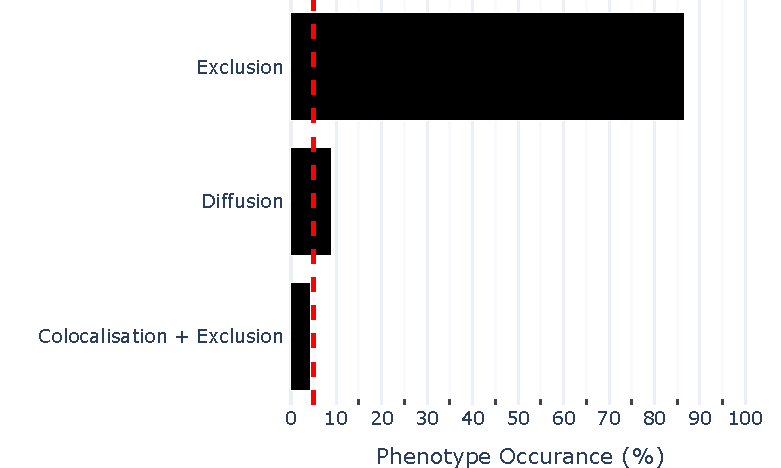
\includegraphics[width=1\linewidth]{08. Chapter 3/Figs/02. Infection/01. IFIT1/04. bar_i1_beas2b.pdf} 
    \end{subfigure}
    \begin{subfigure}{0.495\textwidth}
        \caption{}
        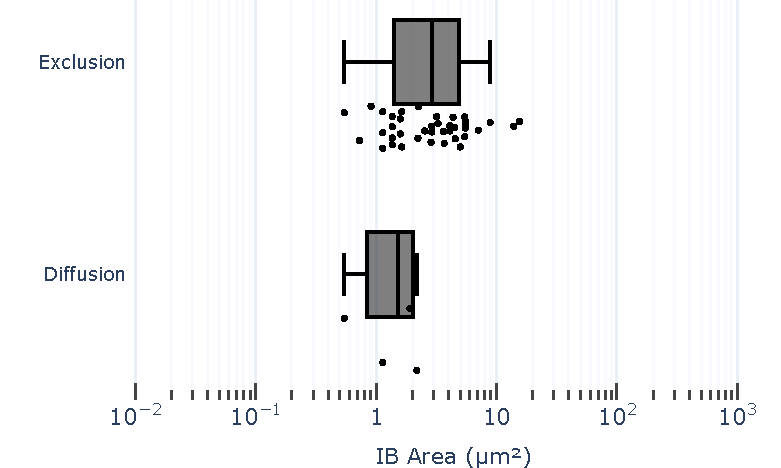
\includegraphics[width=1\linewidth]{08. Chapter 3/Figs/02. Infection/01. IFIT1/05. box_i1_beas2b.pdf}
    \end{subfigure}
    \caption[Phenotypic Diversity of hIFIT1 Interactions with hRSV Inclusion Bodies in BEAS2B Cell Line.]{\textbf{Phenotypic Diversity of hIFIT1 Interactions with hRSV Inclusion Bodies in BEAS2B Cell Line.} BEAS2B cells were infected with human RSV at MOI 1 and fixed 24 HPI. Cells were double-labeled with with anti-RSV N and anti-IFIT1 antibodies and imaged on confocal microscope. Panel (a) shows percentual proportions of observed phenotypes between hRSV inclusion bodies and hIFIT1 (45 observations), with the red dotted line denoting the 5\% threshold, marking phenotypes considered relevant above this limit. Panel (b) shows the IB area in \(\mu \mbox{m}^2\) per observed relevant phenotype.}
    \label{fig:Phenotypic Diversity of hIFIT1 Interactions with hRSV Inclusion Bodies in BEAS2B Cell Line}
\end{figure}

\begin{figure}
    \centering
    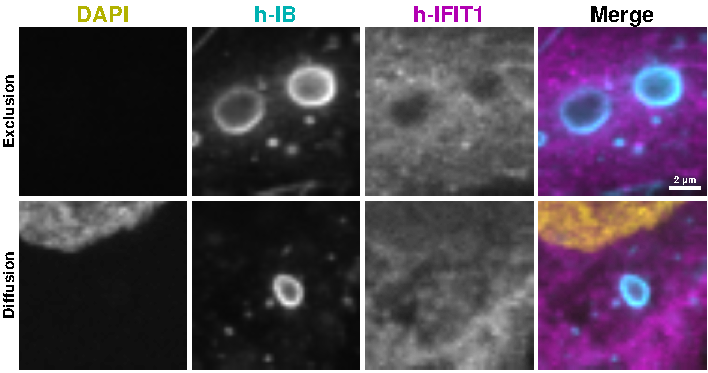
\includegraphics[width=1\linewidth]{08. Chapter 3/Figs/02. Infection/01. IFIT1/06. beas2b i1.pdf}
    \caption[Representative Images of Phenotypic Diversity of hIFIT1 Interactions with hRSV Inclusion Bodies in BEAS2B Cell Line.]{\textbf{Representative Images of Phenotypic Diversity of hIFIT1 Interactions with hRSV Inclusion Bodies in BEAS2B Cell Line.} BEAS2B cells were infected with hRSV at MOI 1 and fixed at 24 HPI. Cellular nuclei were stained with DAPI (yellow), and cells were double-labeled with anti-RSV N (cyan) and anti-IFIT1 (magenta) antibodies. This figure showcases representative examples of relevant phenotypes in the interaction between hIFIT1 and hRSV inclusion bodies. These phenotypes are presented in descending order based on their percentage proportions. The scale bar indicates 2 \(\mu \mbox{m}\).}
    \label{fig:Representative Images of Phenotypic Diversity of hIFIT1 Interactions with hRSV Inclusion Bodies in BEAS2B Cell Line}
\end{figure}

Lastly we investigated the behaviour of bovine IFIT1 during bRSV infection. Figure \ref{fig:Phenotypic Diversity of bIFIT1 Interactions with bRSV Inclusion Bodies in MDBK Cell Line} higlights the phynotipic diversity of 117 observations in detail. Similar to what was observed in A549 and BEAS2B cell line, the most common phenotype with around 65\% frequency is exclusion, however, the second most common one is intra IB inclusion (around 23\%). This is followed by diffusion phenotype, and edge exclusion without or with the presence of possible IBAGs. Out of these, only diffusion was observed with at least 5\% frequency. The representative images of phenotypes with frequency of occurance above 5\% are presented in Figure \ref{fig:Representative Images of Phenotypic Diversity of bIFIT1 Interactions with bRSV Inclusion Bodies in MDBK Cell Line}. In terms of the IB size profile during each observed phenotype, the exclusion-associated IBs had the mean size of 2 \(\mu \mbox{m}\), with the sizes ranging from sub 0.5 \(\mu \mbox{m}\) to supra 30 \(\mu \mbox{m}\), comparable with the median values on overal distribution of the aggregate IB size values detected in MDBK cell line. The inclusion clustered in two size ranges, predominantly to IBs with the size of around 0.9 \(\mu \mbox{m}\), and to IBs with the sizes above 10 \(\mu \mbox{m}\). Lastly, we observed the diffusion phenotype to occur in IBs from 0.2 \(\mu \mbox{m}\) to around 7 \(\mu \mbox{m}\), with the median value of 1.3 \(\mu \mbox{m}\).

COMPARE AND CONTRAST ALL IFIT1 IN ALL 3 CELL LINES

\begin{figure}
    \begin{subfigure}{0.495\textwidth}
        \caption{}
        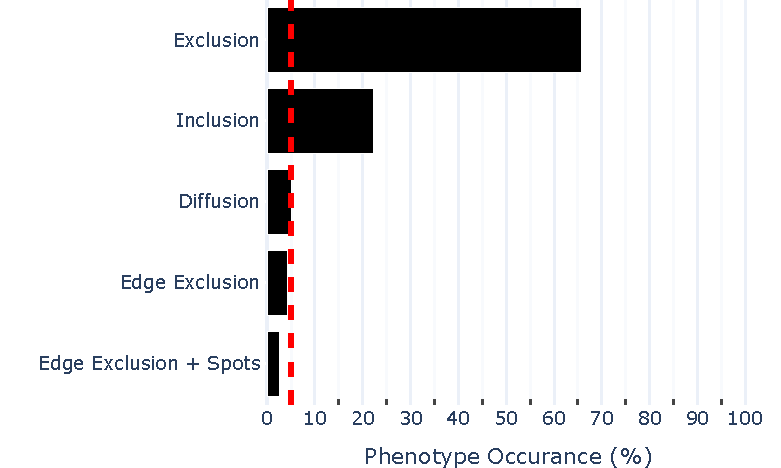
\includegraphics[width=1\linewidth]{08. Chapter 3/Figs/02. Infection/01. IFIT1/07. bar_i1_mdbk.pdf} 
    \end{subfigure}
    \begin{subfigure}{0.495\textwidth}
        \caption{}
        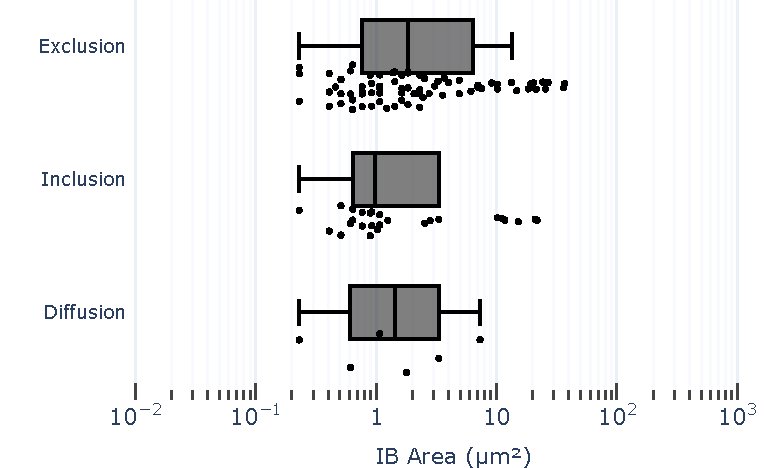
\includegraphics[width=1\linewidth]{08. Chapter 3/Figs/02. Infection/01. IFIT1/08. box_i1_mdbk.pdf}
    \end{subfigure}
    \caption[Phenotypic Diversity of bIFIT1 Interactions with bRSV Inclusion Bodies in MDBK Cell Line.]{\textbf{Phenotypic Diversity of bIFIT1 Interactions with bRSV Inclusion Bodies in MDBK Cell Line.} MDBK cells were infected with bovine RSV at MOI 1 and fixed 24 HPI. Cells were double-labeled with with anti-RSV N and anti-IFIT1 antibodies and imaged on confocal microscope. Panel (a) shows percentual proportions of observed phenotypes between bRSV inclusion bodies and bIFIT1 (117 observations), with the red dotted line denoting the 5\% threshold, marking phenotypes considered relevant above this limit. Panel (b) shows the IB area in \(\mu \mbox{m}^2\) per observed relevant phenotype.}
    \label{fig:Phenotypic Diversity of bIFIT1 Interactions with bRSV Inclusion Bodies in MDBK Cell Line}
\end{figure}

\begin{figure}
    \centering
    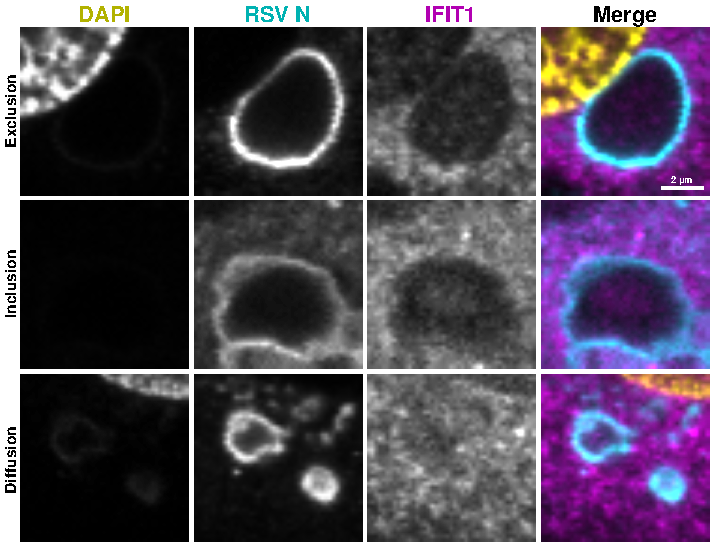
\includegraphics[width=1\linewidth]{08. Chapter 3/Figs/02. Infection/01. IFIT1/09. mdbk i1.pdf}
    \caption[Representative Images of Phenotypic Diversity of bIFIT1 Interactions with bRSV Inclusion Bodies in MDBK Cell Line.]{\textbf{Representative Images of Phenotypic Diversity of bIFIT1 Interactions with bRSV Inclusion Bodies in MDBK Cell Line.} MDBK cells were infected with bRSV at MOI 1 and fixed at 24 HPI. Cellular nuclei were stained with DAPI (yellow), and cells were double-labeled with anti-RSV N (cyan) and anti-IFIT1 (magenta) antibodies. This figure showcases representative examples of relevant phenotypes in the interaction between bIFIT1 and bRSV inclusion bodies. These phenotypes are presented in descending order based on their percentage proportions. The scale bar indicates 2 \(\mu \mbox{m}\).}
    \label{fig:Representative Images of Phenotypic Diversity of bIFIT1 Interactions with bRSV Inclusion Bodies in MDBK Cell Line}
\end{figure}

\subsubsection{Phenotypic Diversity of Nascent IFIT2 Interaction with RSV IBs}
As described in Section \ref{subsec:IFIT Subcellular Localisation During Interferon Induction and RSV Infection}, we utilised two antibodies against IFIT2 protein, which yielded differential results with regards to both subcellular localisation and the interaction phenotype with the RSV IBs. With the latter IFIT2A antibody showed IFIT2 to form intra IB inclusions in A549 cell line, while it show IFIT2 to colocalise with the bRSV IB boundry, while being excluded from this structure. On the other hand, IFIT2B antibody showed exclusion of both human and bovine IFIT2 from the IB structures. We examined these interactions in more detail bellow.

The results of the phenotypic diversity of the 340 interactions of IFIT2 proteins in A549 cell line with hRSV IBs, as detected by the IFIT2A antibody, can be seen in the Figure \ref{fig:Phenotypic Diversity of hIFIT2 Interactions with hRSV Inclusion Bodies, Detected by IFIT2A Antibody in A549 Cell Line}. The examples of the phenotypic interactions are shown in Figure \ref{fig:Representative Images of Phenotypic Diversity of hIFIT2 Interactions with hRSV Inclusion Bodies, Detected by IFIT2A Antibody in A549 Cell Line}. We can see that the most common phenotype, occuring with frequency of around 70\%, is intra IB inclusion. This aligns with our observations from Section \ref{subsec:IFIT Subcellular Localisation During Interferon Induction and RSV Infection} (Figure \ref{fig:The Changes in Subcellular Localisation of Human IFITs in A549 Cells Subjected to hIFNa or hRSV}), however we see additional interactions to occur as well. Colocalisation accompanied by exclusion occurs in 30\% of observations, while an exclusion phenotype occured in 1\% of observations. In terms of the measured areas of the IBs in which the differential interaction phenotypes occure with at least 5\% frequency, we can see that the inclusion and colocalisation accompanied by IB exclusion phenotypes clustered into two almost exclusive groups. The former had the median area of 2.1 \(\mu \mbox{m}\), which was lower than the median area of all A549 IB observations (which had median value of 5 \(\mu \mbox{m}\)), while the latter occured in larger Ibs, with the median size of 9 \(\mu \mbox{m}\). It should be noted that there is a ovelap in terms of the sizes of IBs with either phenotype, however, this data sugegst IFIT2 forming predominantly inclusions in imature IBs with its interaction shifting to IB boundry colocalisation with accompanied IB exclusion in the more mature IBs.

\begin{figure}
    \begin{subfigure}{0.495\textwidth}
        \caption{}
        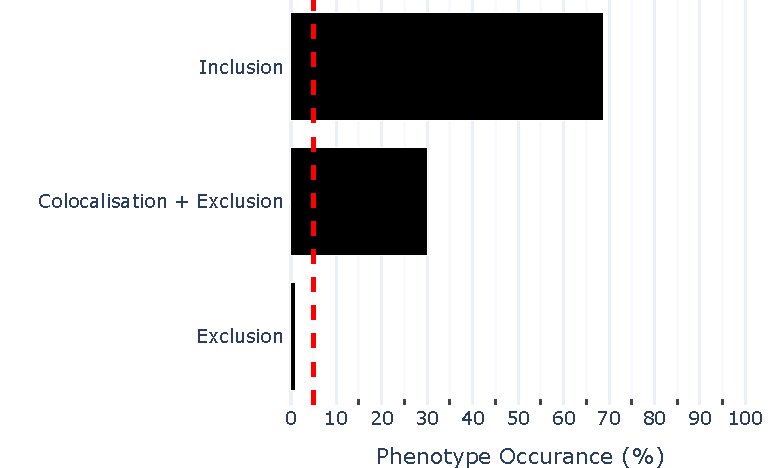
\includegraphics[width=1\linewidth]{08. Chapter 3/Figs/02. Infection/02. IFIT2/01. IFIT2A/01. bar_i2a_a549.pdf}
    \end{subfigure}
    \begin{subfigure}{0.495\textwidth}
        \caption{}
        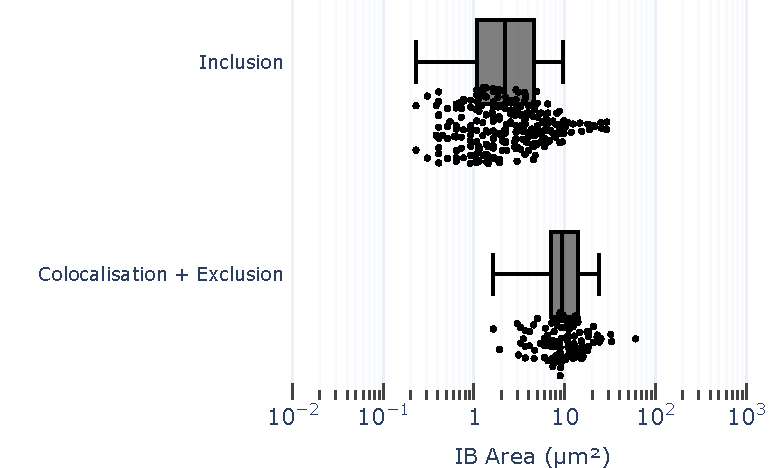
\includegraphics[width=1\linewidth]{08. Chapter 3/Figs/02. Infection/02. IFIT2/01. IFIT2A/02. box_i2a_a549.pdf}
    \end{subfigure}
    \caption[Phenotypic Diversity of hIFIT2 Interactions with hRSV Inclusion Bodies, Detected by IFIT2A Antibody in A549 Cell Line.]{\textbf{Phenotypic Diversity of hIFIT2 Interactions with hRSV Inclusion Bodies, Detected by IFIT2A Antibody in A549 Cell Line.} A549 cells were infected with human RSV at MOI 1 and fixed 24 HPI. Cells were labeled with anti-RSV N and anti-IFIT2A antibodies and imaged on confocal microscope. Panel (a) shows percentual proportions of observed phenotypes between hRSV inclusion bodies and hIFIT2, detected by IFIT2A antibody (340 observations), with the red dotted line denoting the 5\% threshold, marking phenotypes considered relevant above this limit. Panel (b) shows the IB area in \(\mu \mbox{m}^2\) per observed relevant phenotype.}
    \label{fig:Phenotypic Diversity of hIFIT2 Interactions with hRSV Inclusion Bodies, Detected by IFIT2A Antibody in A549 Cell Line}
\end{figure}

\begin{figure}
    \centering
    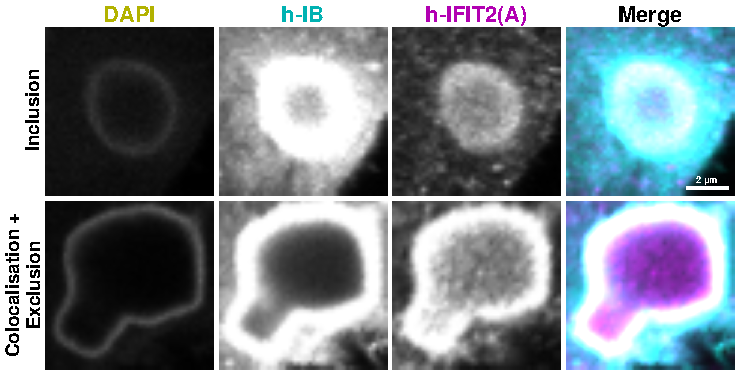
\includegraphics[width=1\linewidth]{08. Chapter 3/Figs/02. Infection/02. IFIT2/01. IFIT2A/03. i2a-a549.pdf}
    \caption[Representative Images of Phenotypic Diversity of hIFIT2 Interactions with hRSV Inclusion Bodies, Detected by IFIT2A Antibody in A549 Cell Line.]{\textbf{Representative Images of Phenotypic Diversity of hIFIT2 Interactions with hRSV Inclusion Bodies, Detected by IFIT2A Antibody in A549 Cell Line.} A549 cells were infected with hRSV at MOI 1 and fixed at 24 HPI. Cellular nuclei were stained with DAPI (yellow), and cells were double-labeled with anti-RSV N (cyan) and anti-IFIT2A (magenta) antibodies. This figure showcases representative examples of relevant phenotypes in the interaction between hIFIT2, detected by IFIT2A antibody, and hRSV inclusion bodies. These phenotypes are presented in descending order based on their percentage proportions. The scale bar indicates 2 \(\mu \mbox{m}\).}
    \label{fig:Representative Images of Phenotypic Diversity of hIFIT2 Interactions with hRSV Inclusion Bodies, Detected by IFIT2A Antibody in A549 Cell Line}
\end{figure}

For IFIT2 interaction phenotypes with hRSV IBs, as detected by the IFIT2B antibody, we observe it to conform to our previous observations from Section \ref{subsec:IFIT Subcellular Localisation During Interferon Induction and RSV Infection} (Figure \ref{fig:The Changes in Subcellular Localisation of Human IFITs in A549 Cells Subjected to hIFNa or hRSV} and Figure \ref{fig:The Changes in Subcellular Localisation of Bovine IFITs in MDBK Cells Subjected to bIFNa or bRSV}). The underlyig phenotype frequence data of these 230 observations, along with the measired IB sizes can be seen in Figure \ref{fig:Phenotypic Diversity of hIFIT2 Interactions with hRSV Inclusion Bodies, Detected by IFIT2B Antibody in A549 Cell Line}, while the representative images of the major occuring phenotype can be seen in Figure \ref{fig:Representative Images of Phenotypic Diversity of hIFIT2 Interactions with hRSV Inclusion Bodies, Detected by IFIT2B Antibody in A549 Cell Line}. We can see that in 97\% of IB occurances, IFIT2 was found to be excluded from the structure. 3\% of the observations showed IFIT2 to be excluded through both cytoplasm and the IB structure. In terms of the size profile of the exclusion-associated IBs, they have a minimal size of 4 \(\mu \mbox{m}^2\), median size of 5 \(\mu \mbox{m}^2\), and maximal observed size of supra 30 \(\mu \mbox{m}^2\). This distribution is neraly identical to the aggregate distribution of all IBs detected in A549 in this study (Section \ref{subsec:IFIT Subcellular Localisation During Interferon Induction and RSV Infection}, Figure \ref{fig:The Distributions of IB Areas Observed Per Cell Line}), which allows us to confirm that IFIT2, as detected by the IFIT2B antibody in A549 cell line, is excluded from these structures regardless of the IB size and thus maturity and these results are not a result of observational bias.

\begin{figure}
    \begin{subfigure}{0.495\textwidth}
        \caption{}
        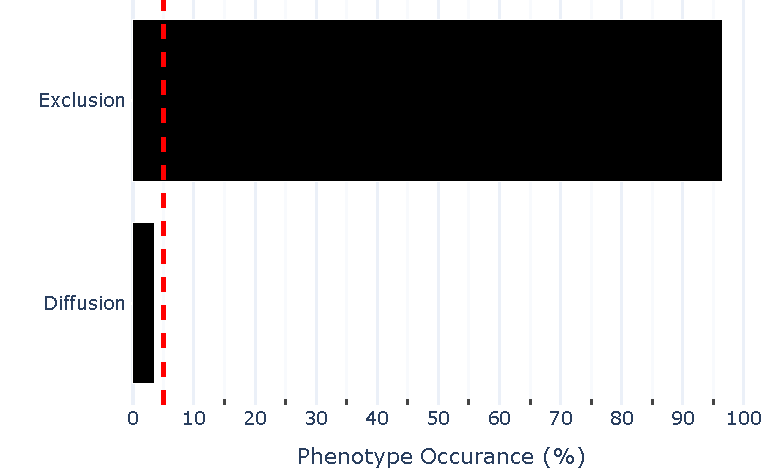
\includegraphics[width=1\linewidth]{08. Chapter 3/Figs/02. Infection/02. IFIT2/02. IFIT2B/01. bar_i2b_a549.pdf}
    \end{subfigure}
    \begin{subfigure}{0.495\textwidth}
        \caption{}
        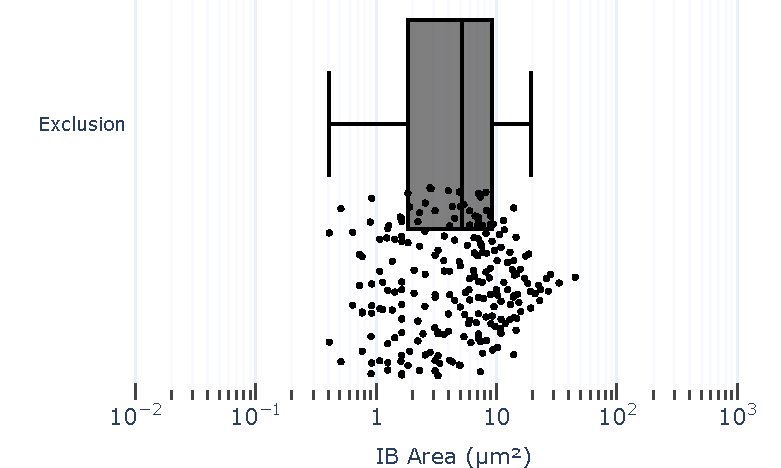
\includegraphics[width=1\linewidth]{08. Chapter 3/Figs/02. Infection/02. IFIT2/02. IFIT2B/02. box_i2b_a549.pdf}
    \end{subfigure}
    \caption[Phenotypic Diversity of hIFIT2 Interactions with hRSV Inclusion Bodies, Detected by IFIT2B Antibody in A549 Cell Line.]{\textbf{Phenotypic Diversity of hIFIT2 Interactions with hRSV Inclusion Bodies, Detected by IFIT2B Antibody in A549 Cell Line.} A549 cells were infected with human RSV at MOI 1 and fixed 24 HPI. Cells were labeled with anti-RSV N and anti-IFIT2B antibodies and imaged on confocal microscope. Panel (a) shows percentual proportions of observed phenotypes between hRSV inclusion bodies and hIFIT2, detected by IFIT2B antibody (230 observations), with the red dotted line denoting the 5\% threshold, marking phenotypes considered relevant above this limit. Panel (b) shows the IB area in \(\mu \mbox{m}^2\) per observed relevant phenotype.}
    \label{fig:Phenotypic Diversity of hIFIT2 Interactions with hRSV Inclusion Bodies, Detected by IFIT2B Antibody in A549 Cell Line}
\end{figure}

\begin{figure}
    \centering
    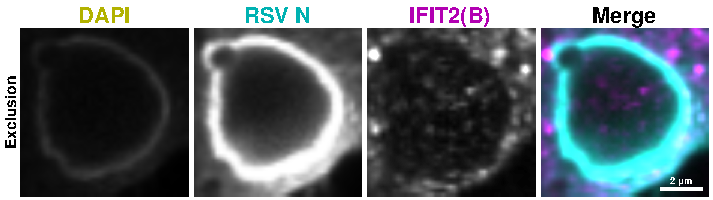
\includegraphics[width=1\linewidth]{08. Chapter 3/Figs/02. Infection/02. IFIT2/02. IFIT2B/03. i2b-a549.pdf} 
    \caption[Representative Images of Phenotypic Diversity of hIFIT2 Interactions with hRSV Inclusion Bodies, Detected by IFIT2B Antibody in A549 Cell Line.]{\textbf{Representative Images of Phenotypic Diversity of hIFIT2 Interactions with hRSV Inclusion Bodies, Detected by IFIT2B Antibody in A549 Cell Line.} A549 cells were infected with hRSV at MOI 1 and fixed at 24 HPI. Cellular nuclei were stained with DAPI (yellow), and cells were double-labeled with anti-RSV N (cyan) and anti-IFIT2B (magenta) antibodies. This figure showcases representative examples of relevant phenotypes in the interaction between hIFIT2, detected by IFIT2B antibody, and hRSV inclusion bodies. These phenotypes are presented in descending order based on their percentage proportions. The scale bar indicates 2 \(\mu \mbox{m}\).}
    \label{fig:Representative Images of Phenotypic Diversity of hIFIT2 Interactions with hRSV Inclusion Bodies, Detected by IFIT2B Antibody in A549 Cell Line}
\end{figure}

Seeing that the IFIT2A antibody showed results of human IFIT2 localisations not observed presiously in our study, while IFIT2B antibody showed results that were consistent with our previous data (both refering to the data from section \ref{subsec:IFIT Subcellular Localisation During Interferon Induction and RSV Infection}, Figure \ref{fig:The Changes in Subcellular Localisation of Human IFITs in A549 Cells Subjected to hIFNa or hRSV}), we decided to validate the IFIT2A results unsing BEA2B cell line infected with hRSV at MOI 1. Smaples were fixed 24 HPI. The phenotipic diversity data can be seen in Figure \ref{fig:Phenotypic Diversity of hIFIT2 Interactions with hRSV Inclusion Bodies, Detected by IFIT2A Antibody in BEAS2B Cell Line}, while the representative images of these phenotypes are shown in Figure \ref{fig:Representative Images of Phenotypic Diversity of hIFIT2 Interactions with hRSV Inclusion Bodies, Detected by IFIT2A Antibody in BEAS2B Cell Line}.

It is to be noted that we had only small amount of observations for this sample (17 observations). Regardless, the results are fairly consistent with the ones from the A549 cell line. We see that the most commonly observed phenotype to be colocalisation accompanied by IB exclusion with the frequency of 59\%, followed by the inclusion phenotype (35\%), and lastly the diffusion phenotype (6\% of observations). Compared to the results from A549 cell line, the two top phenotypes are reversed, although this could be due a bias caused by low sample size. The colocalisation and exclusion phenotype occured in IBs with their sizes raging from sub 1 \(\mu \mbox{m}^2\) to 8 \(\mu \mbox{m}^2\), with the median size of 3 \(\mu \mbox{m}^2\). This is also the median size of IBs from the aggregate of all observations, suggesting this phenotype distributiobn coincise with the overal distribution of IB sizes in BEAS2B cell line 24 HPI. The inclusion and diffucion phenotypes occur in smaller IBs with the median sizes of 1.1 \(\mu \mbox{m}^2\) and 1.3 \(\mu \mbox{m}^2\) respectivelly, with the inclusion phenotype-associated IBs sizes ranging from sub 1 \(\mu \mbox{m}^2\) to 5 \(\mu \mbox{m}^2\).

\begin{figure}
    \begin{subfigure}{0.495\textwidth}
        \caption{}
        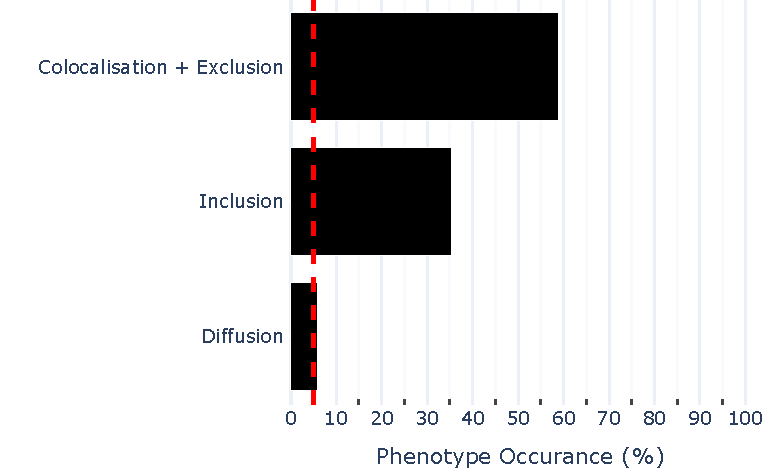
\includegraphics[width=1\linewidth]{08. Chapter 3/Figs/02. Infection/02. IFIT2/01. IFIT2A/10. bar_i2a_beas2b.pdf} 
    \end{subfigure}
    \begin{subfigure}{0.495\textwidth}
        \caption{}
        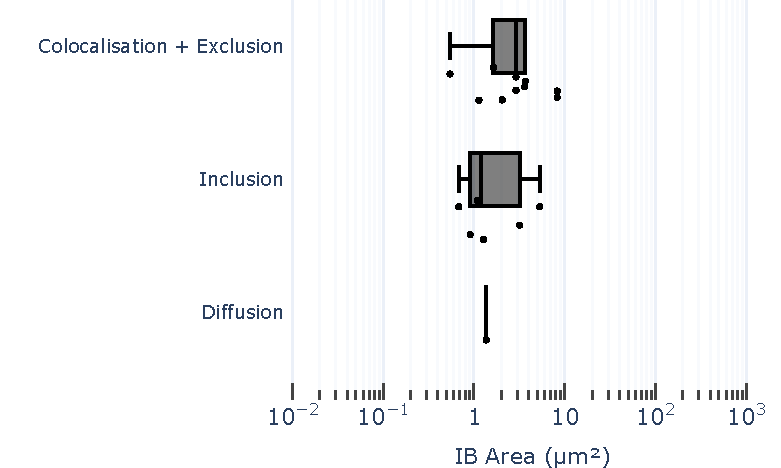
\includegraphics[width=1\linewidth]{08. Chapter 3/Figs/02. Infection/02. IFIT2/01. IFIT2A/11. box_i2a_beas2b.pdf}
    \end{subfigure}
    \caption[Phenotypic Diversity of hIFIT2 Interactions with hRSV Inclusion Bodies, Detected by IFIT2A Antibody in BEAS2B Cell Line.]{\textbf{Phenotypic Diversity of hIFIT2 Interactions with hRSV Inclusion Bodies, Detected by IFIT2A Antibody in BEAS2B Cell Line.} BEAS2B cells were infected with human RSV at MOI 1 and fixed 24 HPI. Cells were labeled with anti-RSV N and anti-IFIT2A antibodies and imaged on confocal microscope. Panel (a) shows percentual proportions of observed phenotypes between hRSV inclusion bodies and hIFIT2, detected by IFIT2A antibody (17 observations), with the red dotted line denoting the 5\% threshold, marking phenotypes considered relevant above this limit. Panel (b) shows the IB area in \(\mu \mbox{m}^2\) per observed relevant phenotype.}
    \label{fig:Phenotypic Diversity of hIFIT2 Interactions with hRSV Inclusion Bodies, Detected by IFIT2A Antibody in BEAS2B Cell Line}
\end{figure}

\begin{figure}
    \centering
    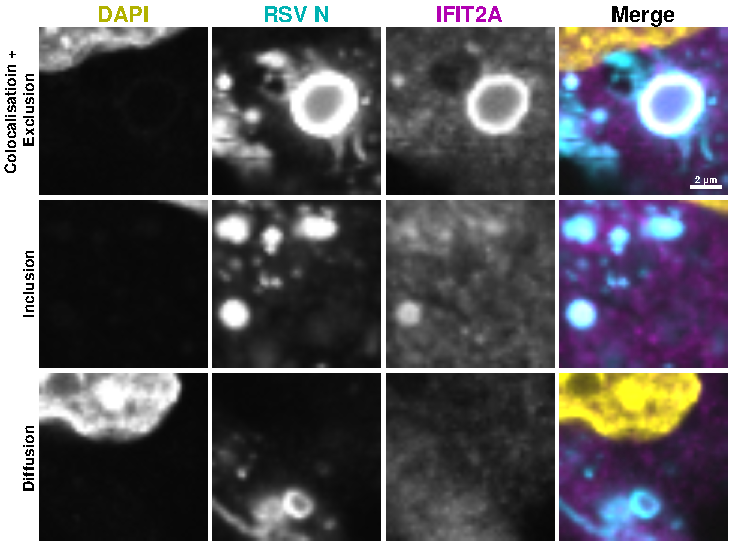
\includegraphics[width=1\linewidth]{08. Chapter 3/Figs/02. Infection/02. IFIT2/01. IFIT2A/12. i2a beas2b.pdf} 
    \caption[Representative Images of Phenotypic Diversity of hIFIT2 Interactions with hRSV Inclusion Bodies, Detected by IFIT2A Antibody in BEAS2B Cell Line.]{\textbf{Representative Images of Phenotypic Diversity of hIFIT2 Interactions with hRSV Inclusion Bodies, Detected by IFIT2A Antibody in BEAS2B Cell Line.} BEAS2B cells were infected with hRSV at MOI 1 and fixed at 24 HPI. Cellular nuclei were stained with DAPI (yellow), and cells were double-labeled with anti-RSV N (cyan) and anti-IFIT2A (magenta) antibodies. This figure showcases representative examples of relevant phenotypes in the interaction between hIFIT2, detected by IFIT2A antibody, and hRSV inclusion bodies. These phenotypes are presented in descending order based on their percentage proportions. The scale bar indicates 2 \(\mu \mbox{m}\).}
    \label{fig:Representative Images of Phenotypic Diversity of hIFIT2 Interactions with hRSV Inclusion Bodies, Detected by IFIT2A Antibody in BEAS2B Cell Line}
\end{figure}

Analysing the phenotipic diversity in 162 observations of bovine IFIT2 intreaction with bRSV IBs in MDBK cell line, as detected by the IFIT2A antibody, we see data consistent with observations in A549 and BEAS2B cell lines. Although in the initial analysis we observed IFIT2 to colocalise with the bRSV IB boundry, we again see two distinct pehotypes occuring, namely the inclusion phenotype (64\% of occurances) and the colocalisation accompanied by exclusion phenotype (36\% of occurances). The IBs associated with these interaction phenotyes had median areas of 0.9 \(\mu \mbox{m}^2\) and 9 \(\mu \mbox{m}^2\) respectively. These data can be seen in Figure \ref{fig:Phenotypic Diversity of bIFIT2 Interactions with bRSV Inclusion Bodies, Detected by IFIT2A Antibody in MDBK Cell Line}, with the representative images of these phenotypes shown in Figure \ref{fig:Representative Images of Phenotypic Diversity of bIFIT2 Interactions with bRSV Inclusion Bodies, Detected by IFIT2A Antibody in MDBK Cell Line}. Similar to what was observed in A549 (Figure \ref{fig:Phenotypic Diversity of hIFIT2 Interactions with hRSV Inclusion Bodies, Detected by IFIT2A Antibody in A549 Cell Line}), the two observed interaction phenotypes cluster in two inner-overlaping clusters, witch suggest these phenotypes are associated with IBs of differential maturity and the inner overlap is a transition phase from one phentope/matiruty stage to another.

\begin{figure}
    \begin{subfigure}{0.495\textwidth}
        \caption{}
        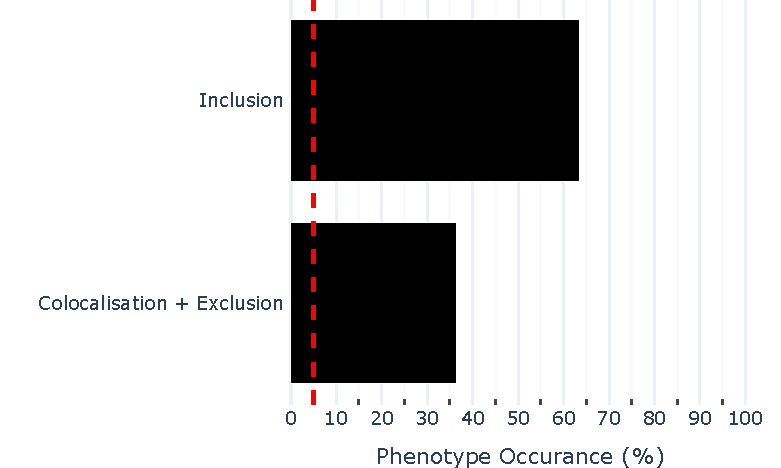
\includegraphics[width=1\linewidth]{08. Chapter 3/Figs/02. Infection/02. IFIT2/01. IFIT2A/13. bar_i2a_mdbk.pdf} 
    \end{subfigure}
    \begin{subfigure}{0.495\textwidth}
        \caption{}
        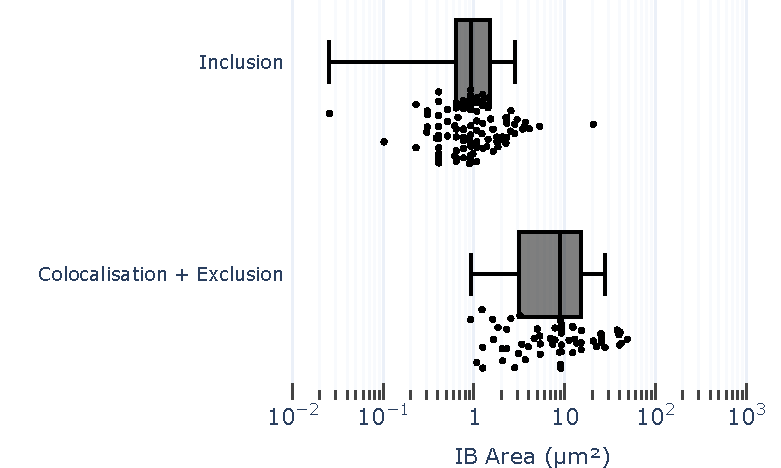
\includegraphics[width=1\linewidth]{08. Chapter 3/Figs/02. Infection/02. IFIT2/01. IFIT2A/14. box_i2a_mdbk.pdf}
    \end{subfigure}
    \caption[Phenotypic Diversity of bIFIT2 Interactions with bRSV Inclusion Bodies, Detected by IFIT2A Antibody in MDBK Cell Line.]{\textbf{Phenotypic Diversity of bIFIT2 Interactions with bRSV Inclusion Bodies, Detected by IFIT2A Antibody in MDBK Cell Line.} MDBK cells were infected with bovine RSV at MOI 1 and fixed 24 HPI. Cells were labeled with anti-RSV N and anti-IFIT2A antibodies and imaged on confocal microscope. Panel (a) shows percentual proportions of observed phenotypes between bRSV inclusion bodies and bIFIT2, detected by IFIT2A antibody (162 observations), with the red dotted line denoting the 5\% threshold, marking phenotypes considered relevant above this limit. Panel (b) shows the IB area in \(\mu \mbox{m}^2\) per observed relevant phenotype.}
    \label{fig:Phenotypic Diversity of bIFIT2 Interactions with bRSV Inclusion Bodies, Detected by IFIT2A Antibody in MDBK Cell Line}
\end{figure}

\begin{figure}
    \centering
    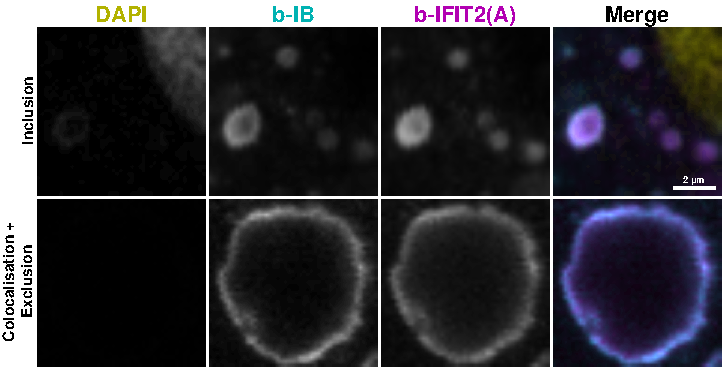
\includegraphics[width=1\linewidth]{08. Chapter 3/Figs/02. Infection/02. IFIT2/01. IFIT2A/15. i2a mdbk brsv.pdf} 
    \caption[Representative Images of Phenotypic Diversity of bIFIT2 Interactions with bRSV Inclusion Bodies, Detected by IFIT2A Antibody in MDBK Cell Line.]{\textbf{Representative Images of Phenotypic Diversity of bIFIT2 Interactions with bRSV Inclusion Bodies, Detected by IFIT2A Antibody in MDBK Cell Line.} MDBK cells were infected with bRSV at MOI 1 and fixed at 24 HPI. Cellular nuclei were stained with DAPI (yellow), and cells were double-labeled with anti-RSV N (cyan) and anti-IFIT2A (magenta) antibodies. This figure showcases representative examples of relevant phenotypes in the interaction between bIFIT2, detected by IFIT2A antibody, and bRSV inclusion bodies. These phenotypes are presented in descending order based on their percentage proportions. The scale bar indicates 2 \(\mu \mbox{m}\).}
    \label{fig:Representative Images of Phenotypic Diversity of bIFIT2 Interactions with bRSV Inclusion Bodies, Detected by IFIT2A Antibody in MDBK Cell Line}
\end{figure}

Lastly, we assayed the phenotipic diversity of 66 observations of bovine IFIT2 with bRSV IBs in MDBK cell line as detected by IFIT2B antibody (Figure \ref{fig:Phenotypic Diversity of hIFIT2 Interactions with bRSV Inclusion Bodies, Detected by IFIT2B Antibody in MDBK Cell Line}, with the representative images shown in Figure \ref{fig:Representative Images of Phenotypic Diversity of hIFIT2 Interactions with bRSV Inclusion Bodies, Detected by IFIT2B Antibody in MDBK Cell Line}). We observed 4 interation phenotypes to occur, namely exlusion (71 \% occurance), IB edge exclusion with intra IB spots (IBAGs; 21\% ocurance), diffusion (6\% occurance), and edge exclusion phenotype without intra IB spots, which occured in only 1\% of observations. When looking at the size profile of the IBs asscociated with the commonly occuring phenotypes (>5\%) we cab see a separation by IB area. The exclusion interaction phenotype happened in IBs with the median size of 2.2 \(\mu \mbox{m}^2\), a value almost equivalent to the median aggregate value observed in MDBK cell line (2 \(\mu \mbox{m}^2\)), suggesting this phenotype is a good proxy for the whole IB population level interaction. The second most common phenotype, edge exclusion with the presence of IBAGs, occured in IBs raging from 0.5 \(\mu \mbox{m}^2\) to supra 20 \(\mu \mbox{m}^2\), with the median value of 7 \(\mu \mbox{m}^2\). Mjaority of the IBs observed to associate with this phenotype were larger than 4 \(\mu \mbox{m}^2\), a size boundry reported to distingush IBAG containing IBs, althout it is to be noted that a considerable proportion of the IBs was smaller than this value, and thus probably IBAG-less. What this means is the intra IB IFIT2 structures we observed seem not to always be IGAGs, if ever. Lastly, the phenotipic interaction where IFIT2 was seen to be equally diffused throught the cutoplasm and the IB structure occured in large IBs with the median size of 15 \(\mu \mbox{m}^2\).

COMPARE AND CONTRAST ALL IFIT2 IN ALL 3 CELL LINES

\begin{figure}
    \begin{subfigure}{0.495\textwidth}
        \caption{}
        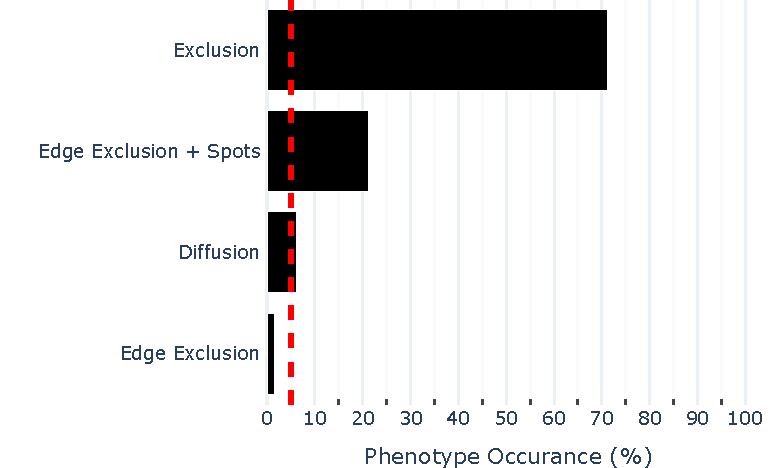
\includegraphics[width=1\linewidth]{08. Chapter 3/Figs/02. Infection/02. IFIT2/02. IFIT2B/10. bar_i2b_mdbk.pdf} 
    \end{subfigure}
    \begin{subfigure}{0.495\textwidth}
        \caption{}
        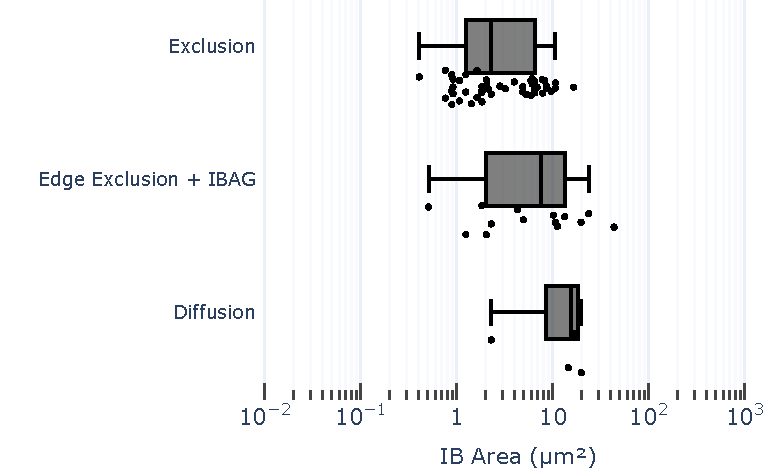
\includegraphics[width=1\linewidth]{08. Chapter 3/Figs/02. Infection/02. IFIT2/02. IFIT2B/11. box_i2b_mdbk.pdf}
    \end{subfigure}
    \caption[Phenotypic Diversity of hIFIT2 Interactions with bRSV Inclusion Bodies, Detected by IFIT2B Antibody in MDBK Cell Line.]{\textbf{Phenotypic Diversity of hIFIT2 Interactions with bRSV Inclusion Bodies, Detected by IFIT2B Antibody in MDBK Cell Line.} MDBK cells were infected with bovine RSV at MOI 1 and fixed 24 HPI. Cells were labeled with anti-RSV N and anti-IFIT2B antibodies and imaged on confocal microscope. Panel (a) shows percentual proportions of observed phenotypes between bRSV inclusion bodies and bIFIT2, detected by IFIT2B antibody (66 observations), with the red dotted line denoting the 5\% threshold, marking phenotypes considered relevant above this limit. Panel (b) shows the IB area in \(\mu \mbox{m}^2\) per observed relevant phenotype.}
    \label{fig:Phenotypic Diversity of hIFIT2 Interactions with bRSV Inclusion Bodies, Detected by IFIT2B Antibody in MDBK Cell Line}
\end{figure}

\begin{figure}
    \centering
    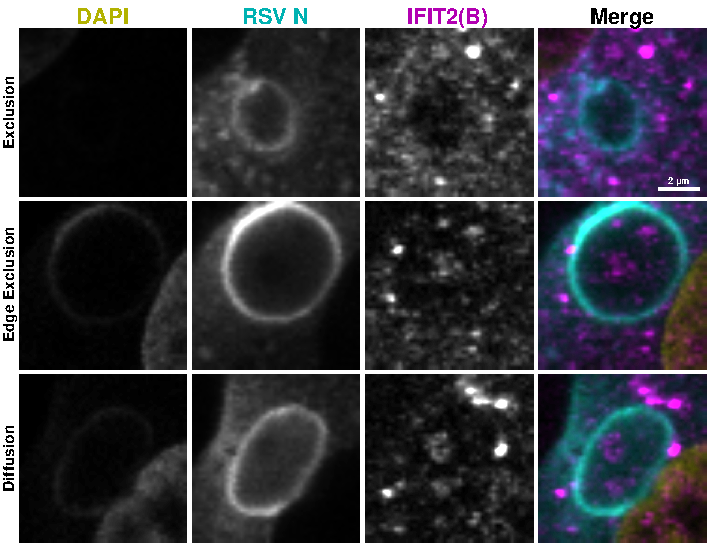
\includegraphics[width=1\linewidth]{08. Chapter 3/Figs/02. Infection/02. IFIT2/02. IFIT2B/12. i2b mdbk brsv.pdf} 
    \caption[Representative Images of Phenotypic Diversity of hIFIT2 Interactions with bRSV Inclusion Bodies, Detected by IFIT2B Antibody in MDBK Cell Line.]{\textbf{Representative Images of Phenotypic Diversity of hIFIT2 Interactions with bRSV Inclusion Bodies, Detected by IFIT2B Antibody in MDBK Cell Line.} MDBK cells were infected with bRSV at MOI 1 and fixed at 24 HPI. Cellular nuclei were stained with DAPI (yellow), and cells were double-labeled with anti-RSV N (cyan) and anti-IFIT2B (magenta) antibodies. This figure showcases representative examples of relevant phenotypes in the interaction between bIFIT2, detected by IFIT2B antibody, and bRSV inclusion bodies. These phenotypes are presented in descending order based on their percentage proportions. The scale bar indicates 2 \(\mu \mbox{m}\).}
    \label{fig:Representative Images of Phenotypic Diversity of hIFIT2 Interactions with bRSV Inclusion Bodies, Detected by IFIT2B Antibody in MDBK Cell Line}
\end{figure}

\subsubsection{Phenotypic Diversity of Nascent IFIT3 Interaction with RSV IBs}
Figure \ref{fig:Phenotypic Diversity of hIFIT3 Interactions with hRSV Inclusion Bodies in A549 Cell Line} shows the frequency of observed phenotypes (panel a) of human IFIT3 interaction with hRSV IBs in A549 cell line, along with the measured areas of the incusion bodies observed per phenotype that occured with at least 5\% frequency (panel b). The representative of the latter are shown in Figure \ref{fig:Representative Images of Phenotypic Diversity of hIFIT3 Interactions with hRSV Inclusion Bodies in A549 Cell Line}. In 54\% out of the 80 total observations, we see human IFIT3 to be excluded from the IB structures. This happens in a range of IB sizes, with the measured areas raging from sub 1 \(\mu \mbox{m}^2\) to supra 50 \(\mu \mbox{m}^2\) and the median area of 4.5 \(\mu \mbox{m}^2\). This distribution is similar to the total aggregate distribution of all IBs observed from A549 cell line. The second most frequent phenotype with 17\% of occurance is the edge exclusion phenotype, where we detect IFIT3 equally distributed between cytoplasm and the IB structure, with the exeption of IB boundry, from which IFIT3 is excluded. This phenotype occurs in more mature IBs with the median size of 12 \(\mu \mbox{m}^2\), although we observed it in a few IBs with measured area of 2 \(\mu \mbox{m}^2\). A very similar phenotype, where the IFIT3 was observed to be diffused evely throught the cytoplasm and IBs, occured at the frequency of 16\%. This was also the phenotype we have observed in our preliminary analysis prevoiusly (Figure \ref{fig:The Changes in Subcellular Localisation of Human IFITs in A549 Cells Subjected to hIFNa or hRSV}). This diffusion phenotype occurs in Ibs with the median size similar to the ones of observed with the exclusion phenotype (5 \(\mu \mbox{m}^2\)), although we haven't observed the diffusion in the IBs of extreme sizes, i.e. in IBs smaller than 2 \(\mu \mbox{m}^2\) and larger than 20 \(\mu \mbox{m}^2\). Lastly, we have observed IFIT3 to interact with the hRSV IBs. This was either by colocalising with the IB boundry accompanied by exclusion from these structures (10\% of observations), or by forming intra-IB incusions (3\% of observations). Since the former surpassed the arbitrary boundry of 5\% frequency, we included it in the IB size analysis. We observed this interaction phenotype in predominantly smaller IBs, with the median size of 1.9 \(\mu \mbox{m}^2\), although this interaction was also detected in larger IBs (circa 7 \(\mu \mbox{m}^2\)).

\begin{figure}
    \begin{subfigure}{0.495\textwidth}
        \caption{}
        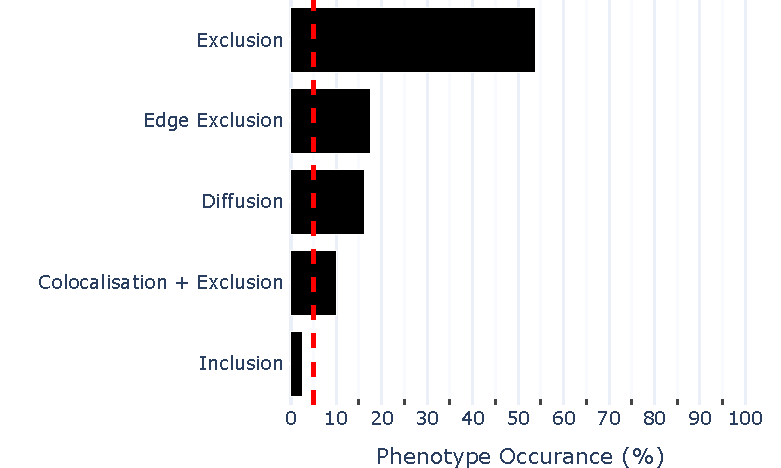
\includegraphics[width=1\linewidth]{08. Chapter 3/Figs/02. Infection/03. IFIT3/01. bar_i3_a549.pdf} 
    \end{subfigure}
    \begin{subfigure}{0.495\textwidth}
        \caption{}
        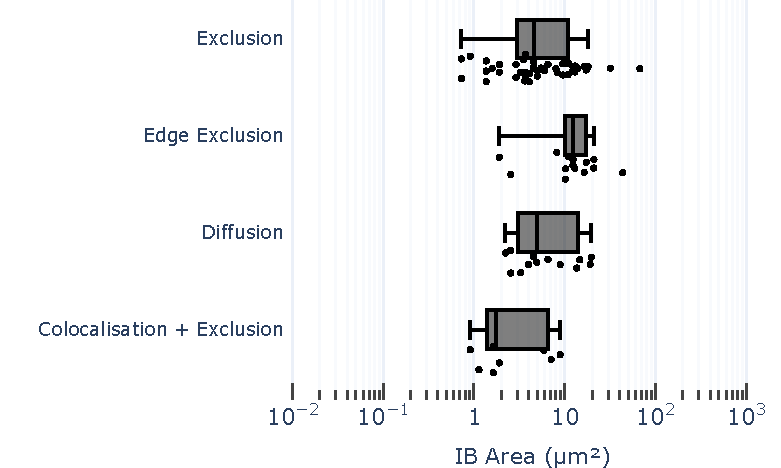
\includegraphics[width=1\linewidth]{08. Chapter 3/Figs/02. Infection/03. IFIT3/02. box_i3_a549.pdf}
    \end{subfigure}
    \caption[Phenotypic Diversity of hIFIT3 Interactions with hRSV Inclusion Bodies in A549 Cell Line.]{\textbf{Phenotypic Diversity of hIFIT3 Interactions with hRSV Inclusion Bodies in A549 Cell Line.} A549 cells were infected with human RSV at MOI 1 and fixed 24 HPI. Cells were double-labeled with with anti-RSV N and anti-IFIT3 antibodies and imaged on confocal microscope. Panel (a) shows percentual proportions of observed phenotypes between hRSV inclusion bodies and hIFIT3 (80 observations), with the red dotted line denoting the 5\% threshold, marking phenotypes considered relevant above this limit. Panel (b) shows the IB area in \(\mu \mbox{m}^2\) per observed relevant phenotype.}
    \label{fig:Phenotypic Diversity of hIFIT3 Interactions with hRSV Inclusion Bodies in A549 Cell Line}
\end{figure}

\begin{figure}
    \centering
    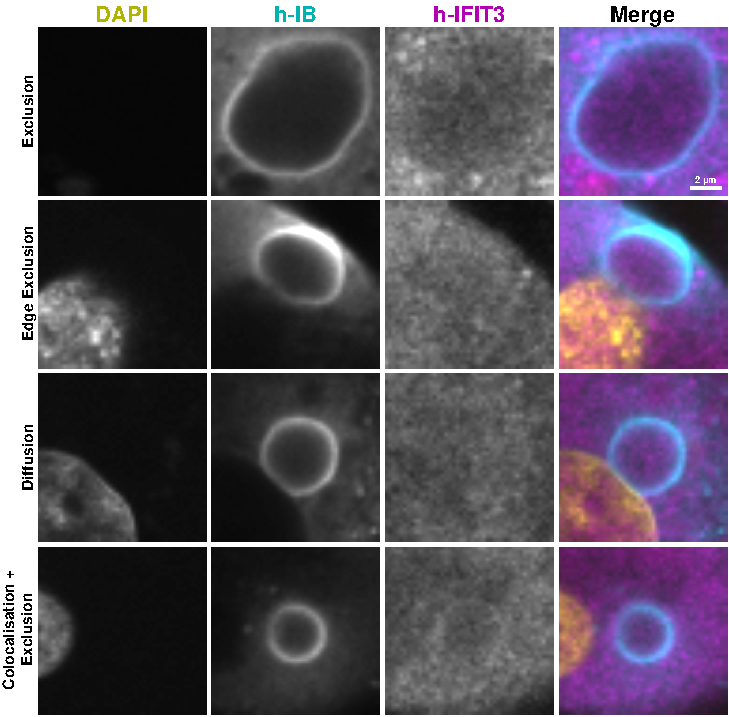
\includegraphics[width=1\linewidth]{08. Chapter 3/Figs/02. Infection/03. IFIT3/03. a549 i3.pdf}
    \caption[Representative Images of Phenotypic Diversity of hIFIT3 Interactions with hRSV Inclusion Bodies in A549 Cell Line.]{\textbf{Representative Images of Phenotypic Diversity of hIFIT3 Interactions with hRSV Inclusion Bodies in A549 Cell Line.} A549 cells were infected with hRSV at MOI 1 and fixed at 24 HPI. Cellular nuclei were stained with DAPI (yellow), and cells were double-labeled with anti-RSV N (cyan) and anti-IFIT3 (magenta) antibodies. This figure showcases representative examples of relevant phenotypes in the interaction between hIFIT3 and hRSV inclusion bodies. These phenotypes are presented in descending order based on their percentage proportions. The scale bar indicates 2 \(\mu \mbox{m}\).}
    \label{fig:Representative Images of Phenotypic Diversity of hIFIT3 Interactions with hRSV Inclusion Bodies in A549 Cell Line}
\end{figure}

To validate this date we looked at the phenotipic diversity of interactions between human IFIT3 and hRSV Ibs in the BEAS2B cell line. The observed phenotypes, along with the calculated occurance frequencies and measured associated IB areas are shown in Figure \ref{fig:Phenotypic Diversity of hIFIT3 Interactions with hRSV Inclusion Bodies in BEAS2B Cell Line}, with the representative images of these phenotypes being shown in Figure \ref{fig:Representative Images of Phenotypic Diversity of hIFIT3 Interactions with hRSV Inclusion Bodies in BEAS2B Cell Line}. Tt is to be noted that we aquired only a small amount of observations (16) from this cell line. Regardless, the obtained data mirrors observations from A549 in all the aspects of the nature of observed phenotypes, the frequency of ocurance of these phenotypes, and the area of IBs associated withthese pehnotypes. In more detail, the most frequent phenotipic interaction was exclusion (62\% of observations), followed by diffusion (19\% of observations), edge exclusion (12\% of observations), and lastly colocalisation with the IB structure (6\% of observations). The median size of IBs associated with the exclusion phenotype was 5.5 \(\mu \mbox{m}^2\), a value which is sligltly higher than the median aggregate value for BEAS2B IBs (3 \(\mu \mbox{m}^2\)). The diffusion phenotype was detected predominantly from smaller IBs with median area of 3 \(\mu \mbox{m}^2\), while the edge exclusion phenotype was observed in IBs with the median size of 10 \(\mu \mbox{m}^2\). Lastly, we have observed one IB-IFIT3 interaction which resulted in colocalisation with the measured IB area of 2.3 \(\mu \mbox{m}^2\). It is remarkable that using such a small number of obersvations mirrors the results from the A549 cell line so well (as can be seen when compared to Figure \ref{fig:Phenotypic Diversity of hIFIT3 Interactions with hRSV Inclusion Bodies in A549 Cell Line}). Overall, this data validates the results obtained from A549 cell line.

\begin{figure}
    \begin{subfigure}{0.495\textwidth}
        \caption{}
        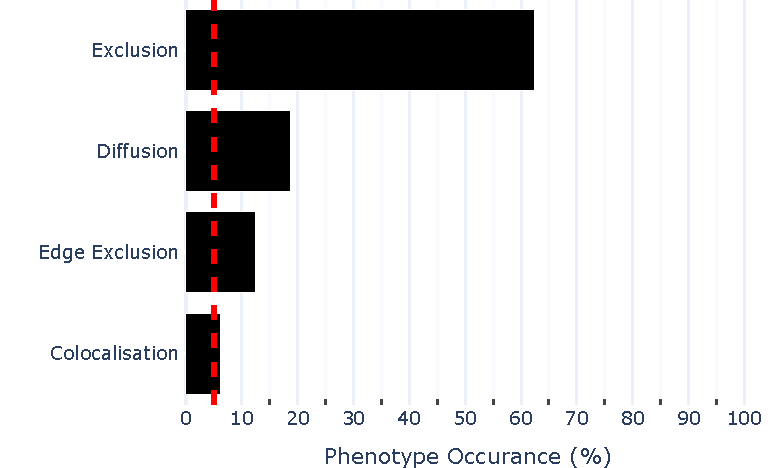
\includegraphics[width=1\linewidth]{08. Chapter 3/Figs/02. Infection/03. IFIT3/04. bar_i3_beas2b.pdf} 
    \end{subfigure}
    \begin{subfigure}{0.495\textwidth}
        \caption{}        
        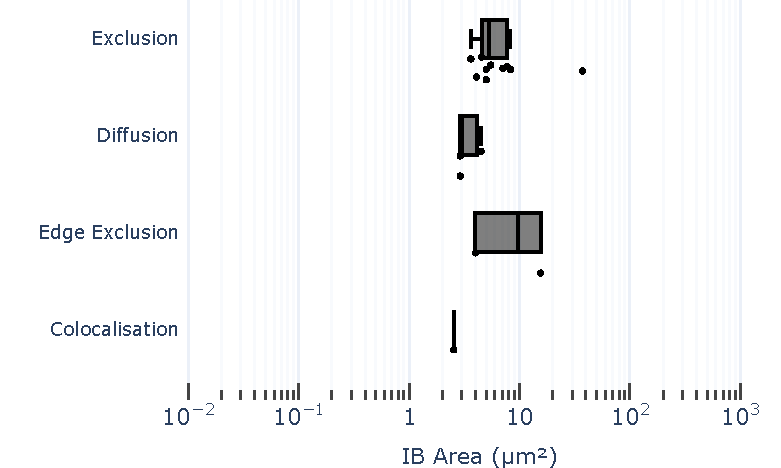
\includegraphics[width=1\linewidth]{08. Chapter 3/Figs/02. Infection/03. IFIT3/05. box_i3_beas2b.pdf}
    \end{subfigure}
    \caption[Phenotypic Diversity of hIFIT3 Interactions with hRSV Inclusion Bodies in BEAS2B Cell Line.]{\textbf{Phenotypic Diversity of hIFIT3 Interactions with hRSV Inclusion Bodies in BEAS2B Cell Line.} BEAS2B cells were infected with human RSV at MOI 1 and fixed 24 HPI. Cells were labeled with anti-RSV N and anti-IFIT3 antibodies and imaged on confocal microscope. Panel (a) shows percentual proportions of observed phenotypes between hRSV inclusion bodies and hIFIT3 (16 observations), with the red dotted line denoting the 5\% threshold, marking phenotypes considered relevant above this limit. Panel (b) shows the IB area in \(\mu \mbox{m}^2\) per observed relevant phenotype.}
    \label{fig:Phenotypic Diversity of hIFIT3 Interactions with hRSV Inclusion Bodies in BEAS2B Cell Line}
\end{figure}

\begin{figure}
    \centering
    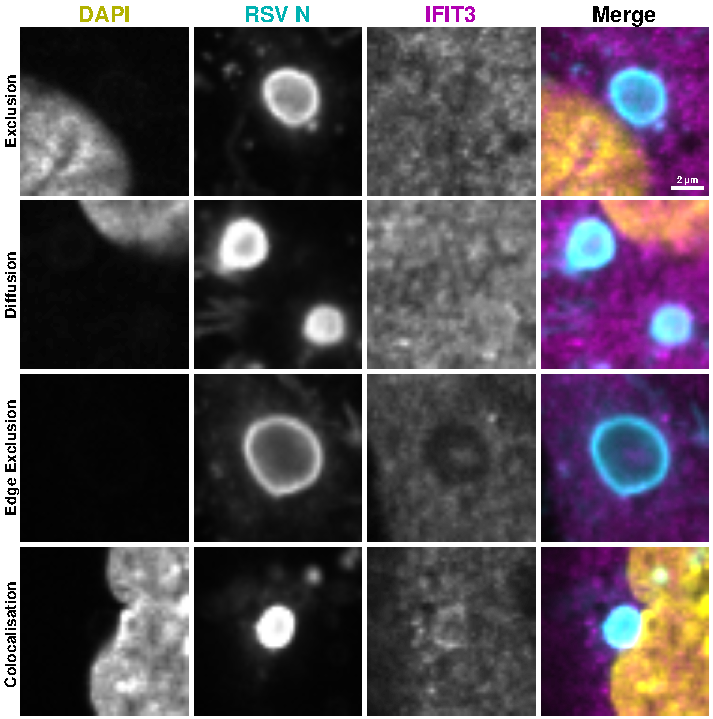
\includegraphics[width=1\linewidth]{08. Chapter 3/Figs/02. Infection/03. IFIT3/06. beas2b i3.pdf}
    \caption[Representative Images of Phenotypic Diversity of hIFIT3 Interactions with hRSV Inclusion Bodies in BEAS2B Cell Line]{\textbf{Representative Images of Phenotypic Diversity of hIFIT3 Interactions with hRSV Inclusion Bodies in BEAS2B Cell Line.} BEAS2B cells were infected with hRSV at MOI 1 and fixed at 24 HPI. Cellular nuclei were stained with DAPI (yellow), and cells were double-labeled with anti-RSV N (cyan) and anti-IFIT3 (magenta) antibodies. This figure showcases representative examples of relevant phenotypes in the interaction between hIFIT3 and hRSV inclusion bodies. These phenotypes are presented in descending order based on their percentage proportions. The scale bar indicates 2 \(\mu \mbox{m}\).}
    \label{fig:Representative Images of Phenotypic Diversity of hIFIT3 Interactions with hRSV Inclusion Bodies in BEAS2B Cell Line}
\end{figure}

Lastly we set to investigate the diversity of interactions between bovine IFIT3 and bRSV IBs in the MDBK cell line, as detected in 214 observations. Previous preliminary analysis suggested that bIFIT3 forms intra-IB inclusions that seem to possess suubstructures resembling IBAGs (Figure \ref{fig:The Changes in Subcellular Localisation of Bovine IFITs in MDBK Cells Subjected to bIFNa or bRSV}). In the more detailed analysis, consisting of 214 observations, we observe the inclusion phenotype to be the second most prevalent interaction phenotype, confirming the prevoius results. The observed phenotypes, along with the calculated occurance frequencies and measured associated IB areas are shown in Figure \ref{fig:Phenotypic Diversity of bIFIT3 Interactions with bRSV Inclusion Bodies in MDBK Cell Line}, with the representative images of these phenotypes being shown in Figure \ref{fig:Representative Images of Phenotypic Diversity of bIFIT3 Interactions with bRSV Inclusion Bodies in MDBK Cell Line}. As observed in A549 and BEAS2B cell lines, the most prevelant interaction between bovine IFIT3 and IBs is exclusion from these structures, which occurs in 43\% of observations. The second most common phenotype is inclusion with 34\% frequency, followed up by diffusion and edge excluison phenotypes, which occured with 12\% and 9\% frequencies respectively. Lastly, we also observed inclusion coocuring with inta IB spots that resemble IBAGs, although only in 2\% of cases. With regards to the IB size profile of categorised based on the different observed phenotypes, we can see that the exclusion, inclusion, and diffusion phenotypes display a similar range of values, ranging from sub 0.5 \(\mu \mbox{m}^2\) to supra 15 \(\mu \mbox{m}^2\), the distribution profile and especially the median values differ between the. While the median values values of exclusion and diffucsion phenotype-associated IBs are shifted towards smaller IBs (1.2 \(\mu \mbox{m}^2\) and 1 \(\mu \mbox{m}^2\) respectively), the median size of 3.3 \(\mu \mbox{m}^2\), above the median aggregate sizes detected in MDBK (2 \(\mu \mbox{m}^2\)). Lastly, the median size of IBs, from which bIFIT3 was observed to be edge excluded, was 11 \(\mu \mbox{m}^2\), acompasing mainly more mature IBs, larger than 3 \(\mu \mbox{m}^2\).

COMPARE AND CONTRAST ALL IFIT3 IN ALL 3 CELL LINES

\begin{figure}
    \begin{subfigure}{0.495\textwidth}
        \caption{}
        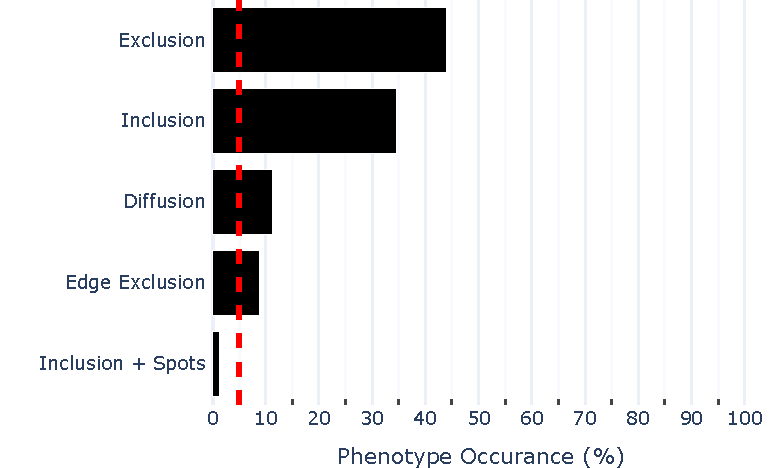
\includegraphics[width=1\linewidth]{08. Chapter 3/Figs/02. Infection/03. IFIT3/07. bar_i3_mdbk.pdf} 
    \end{subfigure}
    \begin{subfigure}{0.495\textwidth}
        \caption{}
        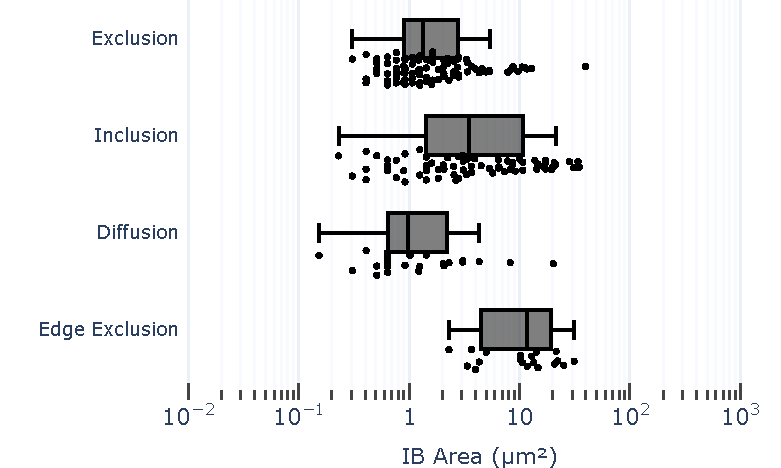
\includegraphics[width=1\linewidth]{08. Chapter 3/Figs/02. Infection/03. IFIT3/08. box_i3_mdbk.pdf}
    \end{subfigure}
    \caption[Phenotypic Diversity of bIFIT3 Interactions with bRSV Inclusion Bodies in MDBK Cell Line.]{\textbf{Phenotypic Diversity of bIFIT3 Interactions with bRSV Inclusion Bodies in MDBK Cell Line.} MDBK cells were infected with bovine RSV at MOI 1 and fixed 24 HPI. Cells were labeled with anti-RSV N and anti-IFIT3 antibodies and imaged on confocal microscope. Panel (a) shows percentual proportions of observed phenotypes between bRSV inclusion bodies and bIFIT3 (214 observations), with the red dotted line denoting the 5\% threshold, marking phenotypes considered relevant above this limit. Panel (b) shows the IB area in \(\mu \mbox{m}^2\) per observed relevant phenotype.}
    \label{fig:Phenotypic Diversity of bIFIT3 Interactions with bRSV Inclusion Bodies in MDBK Cell Line}
\end{figure}

\begin{figure}
    \centering
    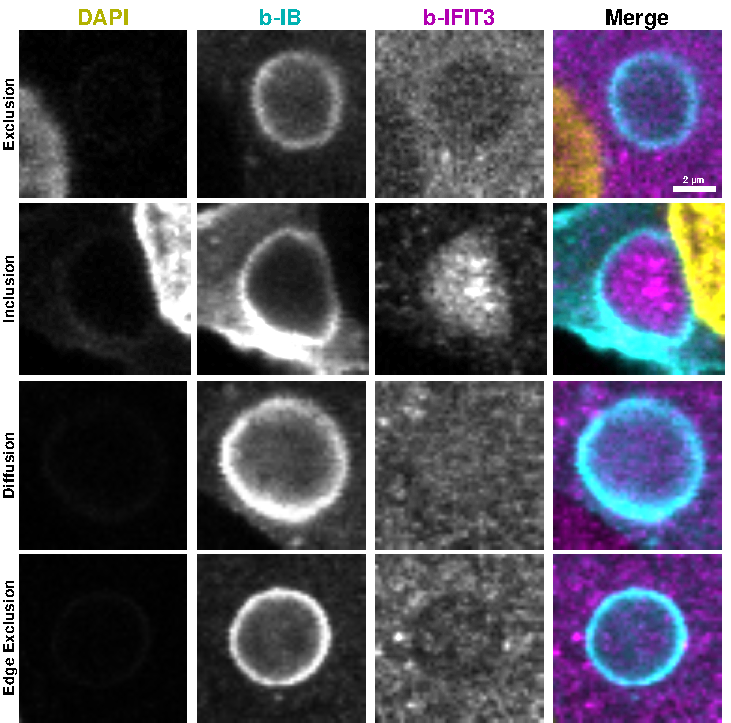
\includegraphics[width=1\linewidth]{08. Chapter 3/Figs/02. Infection/03. IFIT3/09. mdbk i3.pdf}
    \caption[Representative Images of Phenotypic Diversity of bIFIT3 Interactions with bRSV Inclusion Bodies in MDBK Cell Line.]{\textbf{Representative Images of Phenotypic Diversity of bIFIT3 Interactions with bRSV Inclusion Bodies in MDBK Cell Line.} MDBK cells were infected with bRSV at MOI 1 and fixed at 24 HPI. Cellular nuclei were stained with DAPI (yellow), and cells were double-labeled with anti-RSV N (cyan) and anti-IFIT3 (magenta) antibodies. This figure showcases representative examples of relevant phenotypes in the interaction between bIFIT3 and bRSV inclusion bodies. These phenotypes are presented in descending order based on their percentage proportions. The scale bar indicates 2 \(\mu \mbox{m}\).}
    \label{fig:Representative Images of Phenotypic Diversity of bIFIT3 Interactions with bRSV Inclusion Bodies in MDBK Cell Line}
\end{figure}

\subsubsection{Phenotypic Diversity of Nascent IFIT5 Interaction with RSV IBs}
Lastly, we assayed the interactions of human and bovine IFIT5 protien with human and bovine RSV inclusion bodies. Initialy we investigated the diversity of interactions in A549 cell line infected with hRSV at MOI 1 for 24 hours. We assayed 77 observations. Figure \ref{fig:Phenotypic Diversity of hIFIT5 Interactions with hRSV Inclusion Bodies in A549 Cell Line} shows the results of the analysis while Figure \ref{fig:Representative Images of Phenotypic Diversity of hIFIT5 Interactions with hRSV Inclusion Bodies in A549 Cell Line} displays the representative images of interaction phenotypes with the frequency of occurance of at least 5\%. We can see that 57\% of interactions result in exclusion phenotype. This is followed by diffusion and edge exclusion phenotypes, occuring at the frequency of 17\% and 16\% respectively. This were followed by a colocalisation phenotype accompanied by exlusion, which occured in 5\% of observations and was the last interaction phenotype that was included in the IB size analysis. We have however observed 3 more phenotypes, each occuring with only 1\% frequency. These were inclusion, edge exclusion accompanied by possible IBAG presence, and colocalisation phenotypes. With regards to the size profile of IBs associated with the phenotipic interaction that occured with higher than 5\% frequency, exclusion-associated IBs show a distribution similar to the aggegate distribution of all detected IBs in A549 cell line, ranging from sub 1 \(\mu \mbox{m}^2\) to supra 30 \(\mu \mbox{m}^2\) measured areas, with the median value of 6.3 \(\mu \mbox{m}^2\). We can hence assume that this phenotype happens in the whole population of IBs, regardless of the state of maturity. The IBs associated with the diffusion phenotype had median size value of 4 \(\mu \mbox{m}^2\) and were restricted in their maximal size (<10 \(\mu \mbox{m}^2\)). The last two phenotypes, edge excluison and colocalisation accompanied by exclusion, both happened in IBs with sizes larger than 3 \(\mu \mbox{m}^2\), suggesting a certain level of IB maturity was necesarry for these phenotypes to occur. In more detail, edge excluison occured in IBs with the median size of 8 \(\mu \mbox{m}^2\), while the latter had median size of 13 \(\mu \mbox{m}^2\).

\begin{figure}
    \begin{subfigure}{0.495\textwidth}
        \caption{}
        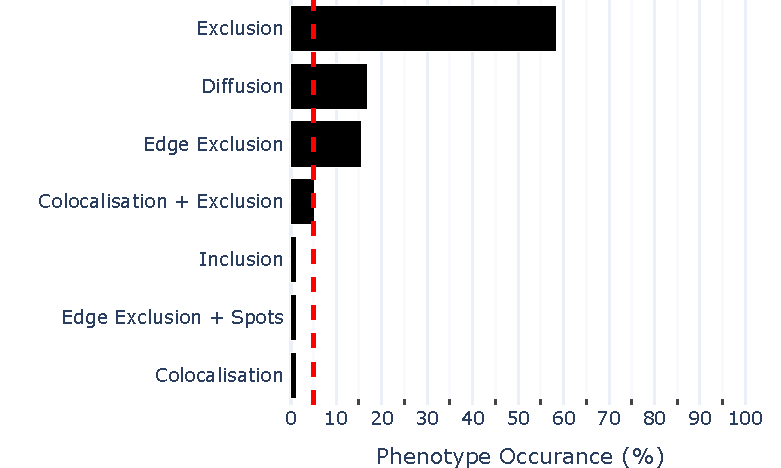
\includegraphics[width=1\linewidth]{08. Chapter 3/Figs/02. Infection/04. IFIT5/01. bar_i5_a549.pdf} 
    \end{subfigure}
    \begin{subfigure}{0.495\textwidth}
        \caption{}
        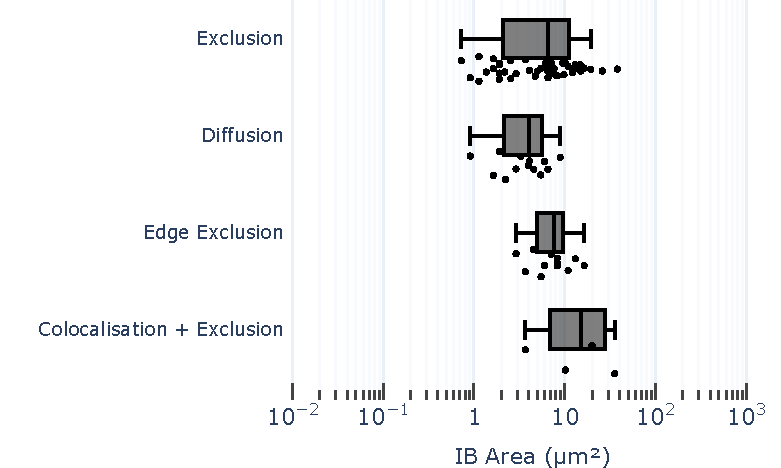
\includegraphics[width=1\linewidth]{08. Chapter 3/Figs/02. Infection/04. IFIT5/02. box_i5_a549.pdf}
    \end{subfigure}
    \caption[Phenotypic Diversity of hIFIT5 Interactions with hRSV Inclusion Bodies in A549 Cell Line.]{\textbf{Phenotypic Diversity of hIFIT5 Interactions with hRSV Inclusion Bodies in A549 Cell Line.} A549 cells were infected with human RSV at MOI 1 and fixed 24 HPI. Cells were labeled with anti-RSV N and anti-IFIT5 antibodies and imaged on confocal microscope. Panel (a) shows percentual proportions of observed phenotypes between hRSV inclusion bodies and hIFIT5 (77 observations), with the red dotted line denoting the 5\% threshold, marking phenotypes considered relevant above this limit. Panel (b) shows the IB area in \(\mu \mbox{m}^2\) per observed relevant phenotype.}
    \label{fig:Phenotypic Diversity of hIFIT5 Interactions with hRSV Inclusion Bodies in A549 Cell Line}
\end{figure}

\begin{figure}
    \centering
    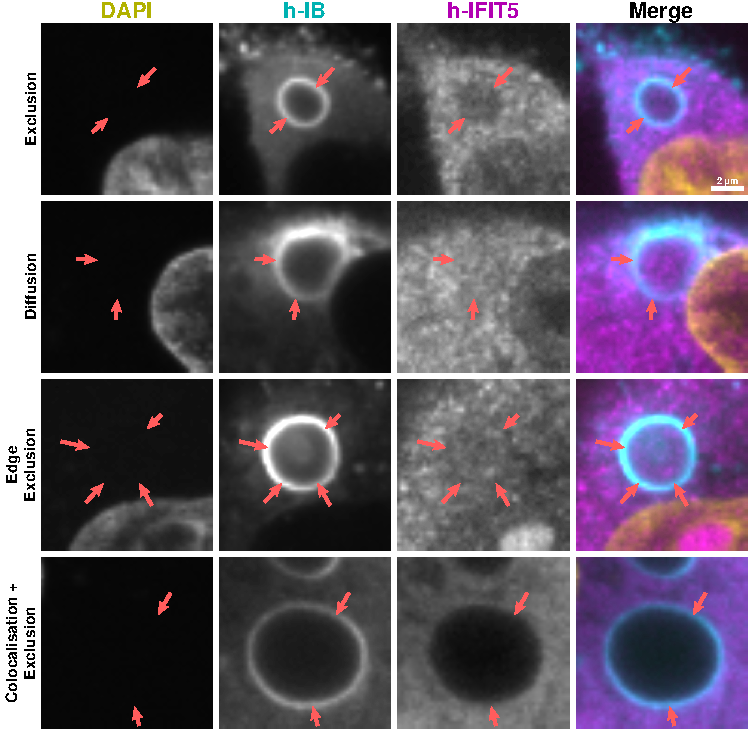
\includegraphics[width=1\linewidth]{08. Chapter 3/Figs/02. Infection/04. IFIT5/03. a549 i5.pdf}
    \caption[Representative Images of Phenotypic Diversity of hIFIT5 Interactions with hRSV Inclusion Bodies in A549 Cell Line.]{\textbf{Representative Images of Phenotypic Diversity of hIFIT5 Interactions with hRSV Inclusion Bodies in A549 Cell Line.} A549 cells were infected with hRSV at MOI 1 and fixed at 24 HPI. Cellular nuclei were stained with DAPI (yellow), and cells were double-labeled with anti-RSV N (cyan) and anti-IFIT5 (magenta) antibodies. This figure showcases representative examples of relevant phenotypes in the interaction between hIFIT5 and hRSV inclusion bodies. These phenotypes are presented in descending order based on their percentage proportions. The scale bar indicates 2 \(\mu \mbox{m}\).}
    \label{fig:Representative Images of Phenotypic Diversity of hIFIT5 Interactions with hRSV Inclusion Bodies in A549 Cell Line}
\end{figure}

We followed this with a validation of these fidings in BEAS2B cell line infected with hRSV. Figure \ref{fig:Phenotypic Diversity of hIFIT5 Interactions with hRSV Inclusion Bodies in BEAS2B Cell Line} shows the results of the analysis while Figure \ref{fig:Representative Images of Phenotypic Diversity of hIFIT5 Interactions with hRSV Inclusion Bodies in BEAS2B Cell Line} displays the representative images of the observed interactions. Although only assesing 21 observations we see similar results to what we observed in A549 cell line. 62\% of IFIT5-hRSV IB observations seem to be excluded from these structures. This is followed by diffusion and edge exclusion phenotypes, both of which appear in 18\% of cases. In terms of the associated IB size profile, all three phenotype median sizes were similar (1.8 \(\mu \mbox{m}^2\), 2.3 \(\mu \mbox{m}^2\), and 3 \(\mu \mbox{m}^2\) respectively), although the exclusion phenotype accompass the largest range of IB sizes (from sub 0.8 \(\mu \mbox{m}^2\) to 10 \(\mu \mbox{m}^2\)). The diffusion-associated IBs clustered in two size ranges, of around 1 \(\mu \mbox{m}^2\) and 4 \(\mu \mbox{m}^2\), while the edge exclusion-associated IBs tended to cluster more close to their median value and did not occure in IBs with extremely small or large values. Overall, although we had a limited amount of observation, this data shows identical results to 92\% of observations from the A549 cell line.

\begin{figure}
    \begin{subfigure}{0.495\textwidth}
        \caption{}
        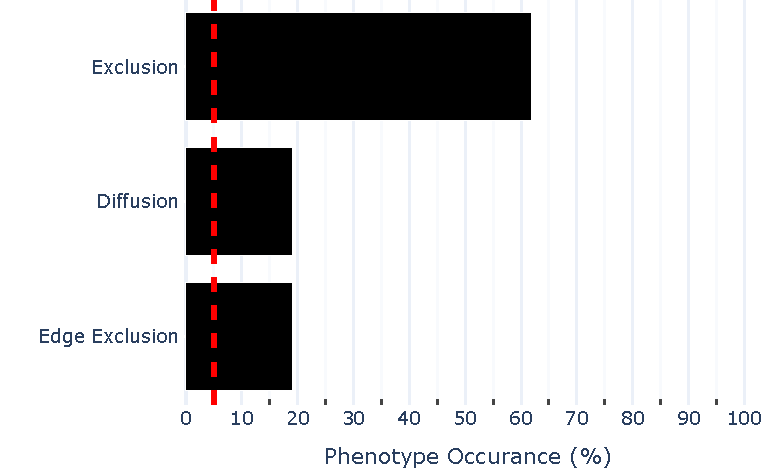
\includegraphics[width=1\linewidth]{08. Chapter 3/Figs/02. Infection/04. IFIT5/04. bar_i5_beas2b.pdf}
    \end{subfigure}
    \begin{subfigure}{0.495\textwidth}
        \caption{}
        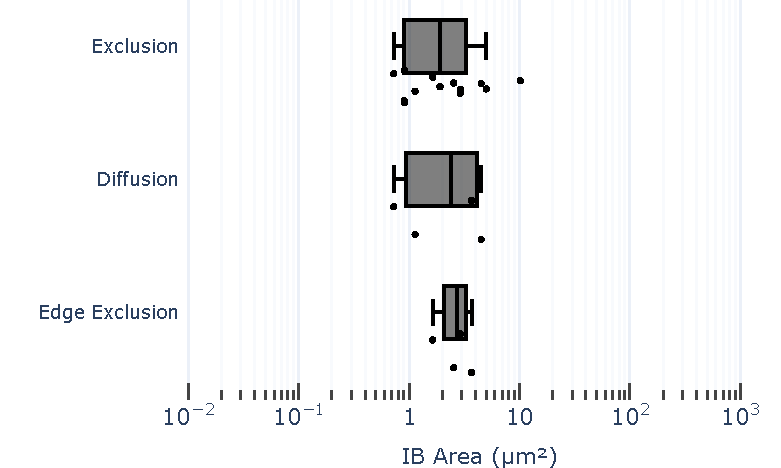
\includegraphics[width=1\linewidth]{08. Chapter 3/Figs/02. Infection/04. IFIT5/05. box_i5_beas2b.pdf}
    \end{subfigure}
    \caption[Phenotypic Diversity of hIFIT5 Interactions with hRSV Inclusion Bodies in BEAS2B Cell Line.]{\textbf{Phenotypic Diversity of hIFIT5 Interactions with hRSV Inclusion Bodies in BEAS2B Cell Line.} BEAS2B cells were infected with human RSV at MOI 1 and fixed 24 HPI. Cells were labeled with anti-RSV N and anti-IFIT5 antibodies and imaged on confocal microscope. Panel (a) shows percentual proportions of observed phenotypes between hRSV inclusion bodies and hIFIT5 (21 observations), with the red dotted line denoting the 5\% threshold, marking phenotypes considered relevant above this limit. Panel (b) shows the IB area in \(\mu \mbox{m}^2\) per observed relevant phenotype.}
    \label{fig:Phenotypic Diversity of hIFIT5 Interactions with hRSV Inclusion Bodies in BEAS2B Cell Line}
\end{figure}

\begin{figure}
    \centering
    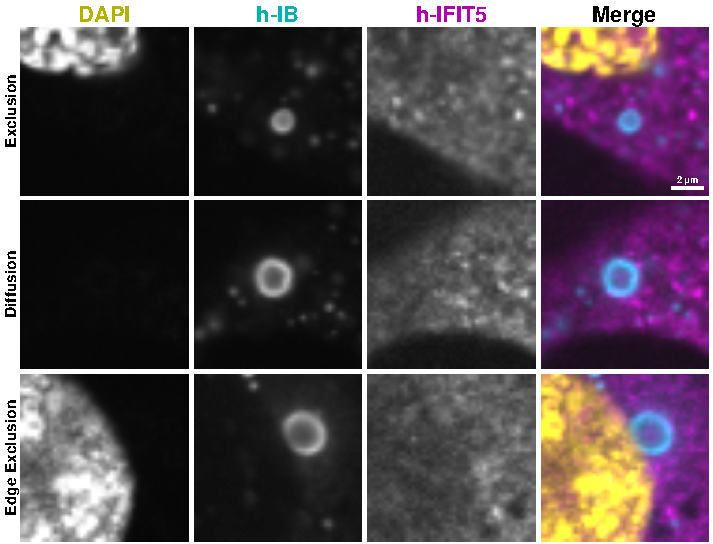
\includegraphics[width=1\linewidth]{08. Chapter 3/Figs/02. Infection/04. IFIT5/06. beas2b i5.pdf}
    \caption[Representative Images of Phenotypic Diversity of hIFIT5 Interactions with hRSV Inclusion Bodies in BEAS2B Cell Line.]{\textbf{Representative Images of Phenotypic Diversity of hIFIT5 Interactions with hRSV Inclusion Bodies in BEAS2B Cell Line.} BEAS2B cells were infected with hRSV at MOI 1 and fixed at 24 HPI. Cellular nuclei were stained with DAPI (yellow), and cells were double-labeled with anti-RSV N (cyan) and anti-IFIT5 (magenta) antibodies. This figure showcases representative examples of relevant phenotypes in the interaction between hIFIT5 and hRSV inclusion bodies. These phenotypes are presented in descending order based on their percentage proportions. The scale bar indicates 2 \(\mu \mbox{m}\).}
    \label{fig:Representative Images of Phenotypic Diversity of hIFIT5 Interactions with hRSV Inclusion Bodies in BEAS2B Cell Line}
\end{figure}

Lastly, we investigated the phenotypes of interactions of bovine IFIT5 with bRSV IBs in MDBK cell line. The percentual frequences of the 61 observations, along with the IB size analysis of the phenotypes occuring more often than 5\% are shown in Figure \ref{fig:Phenotypic Diversity of bIFIT5 Interactions with bRSV Inclusion Bodies in MDBK Cell Line}, with the respreswentative images of the latter shown in Figure \ref{fig:Representative Images of Phenotypic Diversity of bIFIT5 Interactions with bRSV Inclusion Bodies in MDBK Cell Line}. As observed in the human cell lines the exclusion phenotype is the most common (51\% if ibservations), with the sizes of its associated IBs 
raging from sub 0.5 \(\mu \mbox{m}^2\) to supra 20 \(\mu \mbox{m}^2\), although their distribution was sqewed towards sub 3 \(\mu \mbox{m}^2\), with the median area of 1 \(\mu \mbox{m}^2\). This is below the median vaulue of aggregte MDBK IB observations, which had the median size of 2 \(\mu \mbox{m}^2\). Next, edge exclusion, which occured in 29\% of cases, was observed predominantly in large, more mature IBs. Athlough some smaller IBs were observed with this phenotype as well, in general they clustered in line with their median size value of 13 \(\mu \mbox{m}^2\). Contratry to what we observed in the human cell lines previously, the incluson phenotype occurs in 10\% of observations. Inclusion-associated IBs tend to be smaller in size with the median value of 3 \(\mu \mbox{m}^2\), with all of these being smaller than 4 \(\mu \mbox{m}^2\) (with the exeption of one observtion which was 9.5 \(\mu \mbox{m}^2\) in size). Last to observed pheotypes were the diffusion, and edge exclusion co-observed with IBAG-like spots, which occured at 8\% and 2\% respectively. The later was not incuded in the size analysis as it did not occur with a frequency higher than 5\%. For the former, the observed IB sizes associated with this phenotype had a typical size of 0.9 \(\mu \mbox{m}^2\).

PUT ALL CELLINES TOGETHER IFIT5

\begin{figure}
    \begin{subfigure}{0.495\textwidth}
        \caption{}
        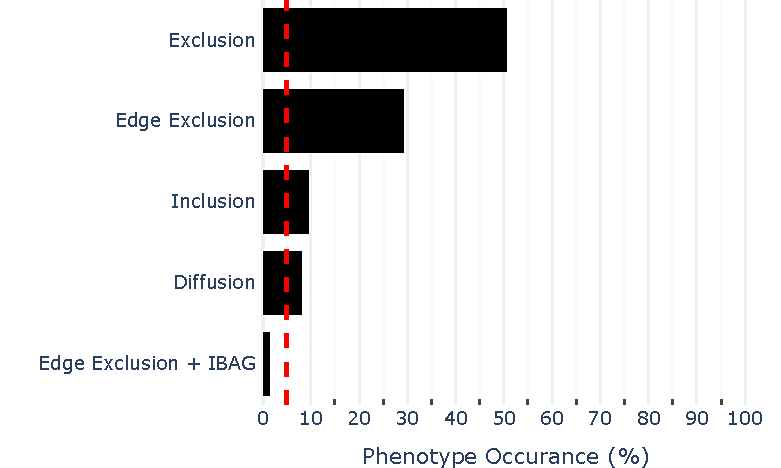
\includegraphics[width=1\linewidth]{08. Chapter 3/Figs/02. Infection/04. IFIT5/07. bar_i5_mdbk.pdf} 
    \end{subfigure}
    \begin{subfigure}{0.495\textwidth}
        \caption{}
        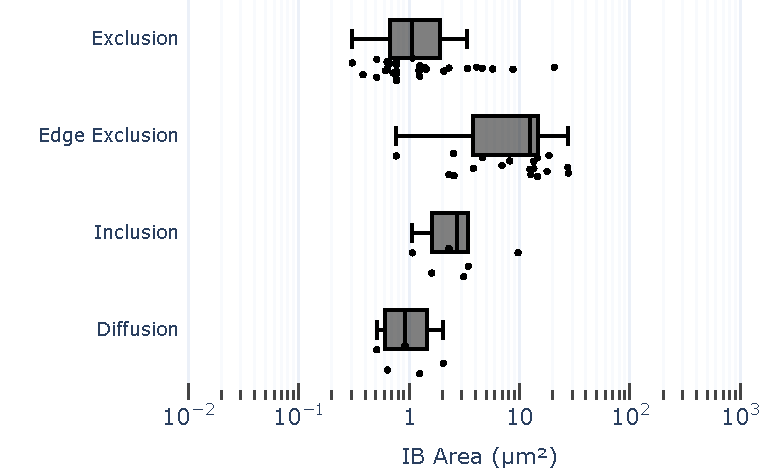
\includegraphics[width=1\linewidth]{08. Chapter 3/Figs/02. Infection/04. IFIT5/08. box_i5_mdbk.pdf}
    \end{subfigure}
    \caption[Phenotypic Diversity of bIFIT5 Interactions with bRSV Inclusion Bodies in MDBK Cell Line.]{\textbf{Phenotypic Diversity of bIFIT5 Interactions with bRSV Inclusion Bodies in MDBK Cell Line.} MDBK cells were infected with bovine RSV at MOI 1 and fixed 24 HPI. Cells were labeled with anti-RSV N and anti-IFIT5 antibodies and imaged on confocal microscope. Panel (a) shows percentual proportions of observed phenotypes between bRSV inclusion bodies and bIFIT5 (61 observations), with the red dotted line denoting the 5\% threshold, marking phenotypes considered relevant above this limit. Panel (b) shows the IB area in \(\mu \mbox{m}^2\) per observed relevant phenotype.}
    \label{fig:Phenotypic Diversity of bIFIT5 Interactions with bRSV Inclusion Bodies in MDBK Cell Line}
\end{figure}

\begin{figure}
    \centering
    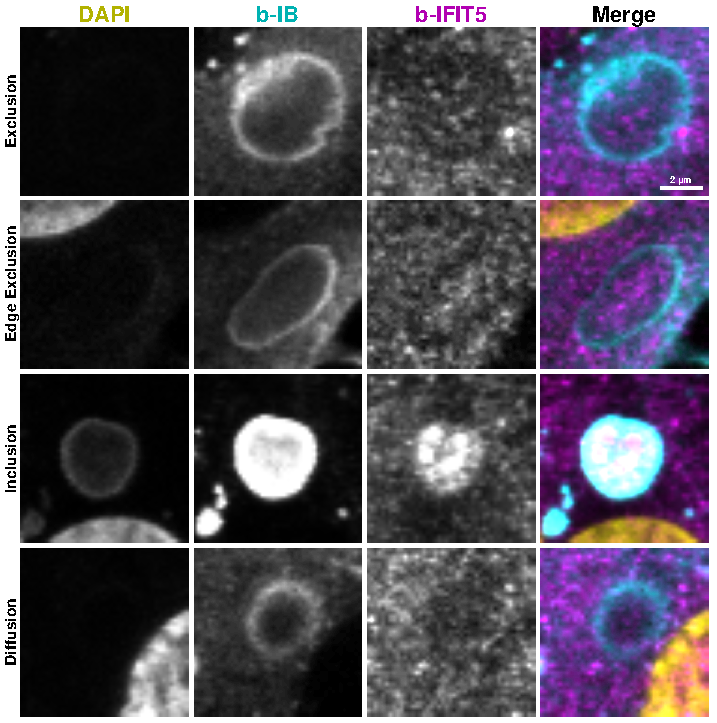
\includegraphics[width=1\linewidth]{08. Chapter 3/Figs/02. Infection/04. IFIT5/09. mdbk i5.pdf}
    \caption[Representative Images of Phenotypic Diversity of bIFIT5 Interactions with bRSV Inclusion Bodies in MDBK Cell Line.]{\textbf{Representative Images of Phenotypic Diversity of bIFIT5 Interactions with bRSV Inclusion Bodies in MDBK Cell Line.} MDBK cells were infected with bRSV at MOI 1 and fixed at 24 HPI. Cellular nuclei were stained with DAPI (yellow), and cells were double-labeled with anti-RSV N (cyan) and anti-IFIT5 (magenta) antibodies. This figure showcases representative examples of relevant phenotypes in the interaction between bIFIT5 and bRSV inclusion bodies. These phenotypes are presented in descending order based on their percentage proportions. The scale bar indicates 2 \(\mu \mbox{m}\).}
    \label{fig:Representative Images of Phenotypic Diversity of bIFIT5 Interactions with bRSV Inclusion Bodies in MDBK Cell Line}
\end{figure}